\documentclass[10pt,journal,final]{IEEEtran}

\usepackage{amsmath,amssymb,amsfonts,amsthm}
\usepackage{algorithm}
\usepackage{algorithmic}
\usepackage{graphicx}
\usepackage{textcomp}
\usepackage{xcolor}
\usepackage{booktabs}
\usepackage{multirow}
\usepackage{cite}
\usepackage{url}
\usepackage{tikz}
\usetikzlibrary{arrows.meta,positioning,shapes.geometric,fit,calc,backgrounds}
\usepackage{microtype}

\newtheorem{theorem}{Theorem}
\newtheorem{proposition}{Proposition}
\newtheorem{lemma}{Lemma}
\newtheorem{remark}{Remark}

\graphicspath{{figures/}}

\begin{document}

\title{Dissecting Continuous-State and Variational Inductive Biases in State Space Duality: An Empirical Audit of Native Mamba-2 Cross-Modal Alignment}

\author{Abhinav~Sai~M.%
\thanks{Manuscript submitted for peer review. Code, audited logs, and configuration artifacts are publicly available at \protect\url{https://github.com/abhinavsai2006/PH_SSD}. (Email: \protect\url{abhinavsai2006@gmail.com})}%
\thanks{The author is with the Department of Computer Science and Engineering.}%
}

\markboth{Journal Submission Draft: Native Mamba-2 Cross-Modal Alignment Audit}%
{M.: Dissecting Continuous-State and Variational Inductive Biases in State Space Duality}

\maketitle

\begin{abstract}
Structured State Space Models (SSMs) and their duality with structured attention---principally embodied in Mamba-2 via State Space Duality (SSD)---offer linear time complexity $O(L)$ with respect to sequence length, presenting an appealing alternative to quadratic self-attention in cross-modal vision-language alignment. In this paper, we conduct a rigorous, pre-registered empirical audit investigating whether continuous-time dynamical system adaptations and variational latent coupling enhance or compromise cross-modal representations built upon frozen vision (ViT-B/16) and language (RoBERTa-base) encoders. We formalize and evaluate three mechanisms: (1) Structure-Aware Hamiltonian-Inspired Dissipative Coordinate-Momentum Adapter (HEDO), incorporating exact skew-symmetric learned interactions $\mathbf{J} = (\mathbf{A} - \mathbf{A}^T)/\sqrt{d}$ and positive diagonal damping $\mathbf{R}$; (2) Adaptive Variational State Coupling (AVSC), which introduces confidence-gated symmetric Kullback-Leibler (KL) divergence across intermediate chunk-boundary states; and (3) Multi-Scale State Aggregation (MSA), fusing global mean, boundary, and terminal recurrent states. Across an audited 24-run, 8-configuration ablation benchmark (three random seeds per configuration, $n=3$ paired runs) on Flickr8k, empirical hypothesis testing indicates: (i) Mamba-2 equipped with HEDO shows no statistically significant difference from the standard linear alignment baseline under the present three-seed evaluation ($37.31 \pm 0.68\%$ vs. $37.16 \pm 0.57\%$ Mean Recall, paired $\Delta = +0.15$ percentage points [pp], 95\% CI $[-1.42, +1.73]$ pp, CI includes zero) while processing $7,054$ pairs/s at the head with $1,086$ MB peak VRAM; (ii) Multi-scale recurrent aggregation consistently degrades retrieval performance ($\Delta \approx -10.27$ to $-10.75$ pp, with 95\% CIs strictly negative), revealing that causal boundary states introduce severe temporal asymmetry that corrupts isotropic pooling; and (iii) Variational coupling is associated with severe alignment degradation ($\Delta \approx -30.52$ to $-32.11$ pp down to a low-retrieval regime of $\approx 5.0\%-6.6\%$), consistent with dimensional collapse under the evaluated formulation. We present geometric and gradient analyses showing that isotropic Gaussian KL penalties conflict with hyperspherical multi-positive InfoNCE contrastive repulsion, providing a mechanistic explanation consistent with this degradation. Our findings deliver vital negative results and actionable design principles for integrating state space duality into multimodal systems.
\end{abstract}

\begin{IEEEkeywords}
Cross-modal retrieval, state space models, Mamba-2, State Space Duality, multimodal representation learning, contrastive learning, Hamiltonian dynamics, variational coupling.
\end{IEEEkeywords}

\IEEEpeerreviewmaketitle

% =========================================================================
% SECTION I: INTRODUCTION
% =========================================================================
\section{Introduction}
\label{sec:introduction}

\IEEEPARstart{C}{ross-modal} vision-language retrieval requires mapping high-dimensional visual patch tokens and textual wordpiece sequences into a geometrically unified semantic metric space~\cite{radford2021learning,wang2016comprehensive}. While Transformer-based architectures parameterized by multi-head self-attention (MHSA) have long dominated this domain~\cite{vaswani2017attention,dosovitskiy2021image,liu2019roberta}, their quadratic computational and memory footprint $O(L^2)$ presents significant scalability bottlenecks for long sequence processing, dense feature maps, and real-time edge retrieval.

To circumvent this limitation, Structured State Space Models (SSMs)---notably S4~\cite{gu2022efficiently}, Mamba~\cite{gu2023mamba}, and Mamba-2~\cite{dao2024transformers}---have emerged as a compelling paradigm. Mamba-2, in particular, formalizes \textit{State Space Duality} (SSD), establishing a mathematical equivalence between continuous-time linear time-varying dynamical systems and 1-semiseparable matrix transformations. By computing recurrence within discrete chunk boundaries and utilizing efficient matrix multiplications, SSD achieves strict $O(L)$ linear sequence scaling while maintaining expressive representational capabilities.

Concurrently, there has been widespread theoretical enthusiasm for incorporating continuous-time dynamical system inductive biases into deep architectures~\cite{greydanus2019hamiltonian,vanderschaft2000}. Hamiltonian neural networks and port-Hamiltonian systems provide energy-conserving coordinate-momentum symplectic geometry, while dissipative damping offers asymptotic stability. In parallel, variational information bottlenecks and variational cross-modal coupling have been widely proposed to enforce smooth, noise-robust latent distributions~\cite{kingma2014auto,alemi2017deep}.

\subsection{Problem Statement}
Despite theoretical promise, an essential question remains unaddressed:
\begin{quote}
\textit{Do continuous-state Hamiltonian adaptations and variational state coupling improve cross-modal alignment when integrated with Native Mamba-2, or can these inductive biases introduce optimization and representation failures?}
\end{quote}

\subsection{Research Gap}
In the existing literature, continuous-time and variational inductive biases are frequently evaluated under isolated, non-audited configurations lacking multi-seed paired-difference hypothesis testing or systematic factorial isolation of individual components. Crucially, the interaction between sequential SSM recurrent dynamics and hyperspherical contrastive alignment manifolds has not been systematically investigated. Without rigorous factorial controls, it is impossible to determine whether reported performance variations stem from the underlying state-space sequence model, continuous-time dynamical adapters, or stochastic optimization noise.

\subsection{Research Questions and Hypotheses}
To resolve this gap, we formalize four pre-registered research questions:
\begin{itemize}
    \item \textbf{RQ1}: Does the integration of a Hamiltonian-inspired dissipative coordinate-momentum adapter (HEDO) preserve or enhance retrieval performance over standard linear alignment?
    \item \textbf{RQ2}: Does multi-scale state aggregation (MSA) combining boundary and terminal recurrent states improve cross-modal representation quality?
    \item \textbf{RQ3}: Does intermediate adaptive variational state coupling (AVSC) improve cross-modal alignment through latent distribution regularization?
    \item \textbf{RQ4}: What are the computational complexity, peak memory footprint, and throughput tradeoffs introduced by these mechanisms?
\end{itemize}

\subsection{Contributions}
In addressing these questions, this paper delivers four primary contributions:
\begin{enumerate}
    \item \textbf{Structured HEDO Adapter Integration}: We design and formalize a Structure-Aware Hamiltonian-Inspired Dissipative Coordinate-Momentum Adapter (HEDO) integrated with Native Mamba-2, establishing energy boundedness under continuous dynamics.
    \item \textbf{Controlled Empirical Audit}: We construct a controlled 8-configuration ablation matrix isolating HEDO, MSA, and AVSC upon strictly frozen ViT-B/16 and RoBERTa-base backbones.
    \item \textbf{Paired Multi-Seed Statistical Evaluation}: Across 24 audited runs (3 independent random seeds per configuration, $n=3$ paired runs), we apply paired Student-$t$ hypothesis testing with 95\% confidence intervals, finding that no statistically significant difference from the baseline was detected for Mamba-2 + HEDO under this sample size ($+0.15$ pp, 95\% CI $[-1.42, +1.73]$ pp).
    \item \textbf{Mechanistic Analysis}: We provide mathematical and gradient analyses explaining how causal boundary states in MSA introduce temporal asymmetry that degrades isotropic pooling ($\approx -10.5$ pp), and show how isotropic Gaussian KL penalties in AVSC conflict with hyperspherical InfoNCE repulsion, providing a mechanistic explanation consistent with dimensional collapse under the evaluated formulation ($\approx -31$ pp).
\end{enumerate}

\subsection{Paper Organization}
The remainder of this paper is organized as follows: Section~\ref{sec:related_work} reviews related literature across state-space models, cross-modal retrieval, and physics-informed architectures. Section~\ref{sec:formulation} establishes the formal problem formulation and hypotheses. Section~\ref{sec:architecture} details the proposed architecture, mathematical formulations, and training algorithm. Section~\ref{sec:methodology} describes the experimental methodology, ablation configurations, and auditing protocol. Section~\ref{sec:results} presents the empirical results, efficiency benchmarks, and statistical tests. Section~\ref{sec:discussion} provides mechanistic failure analyses and practical design guidelines. Section~\ref{sec:limitations} discusses limitations, and Section~\ref{sec:conclusion} concludes the paper.

% =========================================================================
% SECTION II: RELATED WORK
% =========================================================================
\section{Related Work}
\label{sec:related_work}

\subsection{Structured State Space Models}
State Space Models parameterize continuous-time dynamical systems mapping a 1D input signal $x(t) \in \mathbb{R}$ to an output $y(t) \in \mathbb{R}$ through an implicit latent state $\mathbf{h}(t) \in \mathbb{R}^N$:
\begin{equation}
\label{eq:continuous_ssm}
\frac{d\mathbf{h}(t)}{dt} = \mathbf{A}(t)\mathbf{h}(t) + \mathbf{B}(t)x(t), \quad y(t) = \mathbf{C}(t)\mathbf{h}(t) + \mathbf{D}(t)x(t),
\end{equation}
where $\mathbf{A}(t) \in \mathbb{R}^{N \times N}$ represents the state transition matrix, $\mathbf{B}(t) \in \mathbb{R}^{N \times 1}$ is the input projection matrix, $\mathbf{C}(t) \in \mathbb{R}^{1 \times N}$ is the output projection matrix, and $\mathbf{D}(t) \in \mathbb{R}$ represents the direct feedthrough skip connection.

The Structured State Space sequence model (S4)~\cite{gu2022efficiently} stabilized recurrent training by constraining $\mathbf{A}$ to HiPPO (High-order Polynomial Projection Operators) diagonal-plus-low-rank structures. Mamba~\cite{gu2023mamba} introduced data-dependent input-selective parameterization ($\mathbf{B}(t), \mathbf{C}(t), \Delta(t)$), enabling the model to selectively propagate or filter out information along sequence dimensions. 

Most recently, Dao and Gu~\cite{dao2024transformers} introduced Mamba-2, which formalizes \textit{State Space Duality} (SSD), establishing a theoretical equivalence between continuous-time linear time-varying dynamical systems and 1-semiseparable matrix transformations. For a scalar diagonal state transition $A$, the transformation across an input sequence $\mathbf{x} \in \mathbb{R}^L$ is expressed as:
\begin{equation}
\label{eq:ssd_matrix}
\mathbf{y} = \mathbf{M}\mathbf{x}, \quad M_{i,j} = C_i \left( \prod_{k=j+1}^i A_k \right) B_j \quad (i \ge j),
\end{equation}
where $\mathbf{M} \in \mathbb{R}^{L \times L}$ is a lower-triangular 1-semiseparable matrix whose subdiagonal entries factorize into cumulative state transition products. By computing recurrence within discrete chunk boundaries and computing intra-chunk transformations via matrix multiplications on tensor cores, SSD unifies recurrent SSMs and linear attention into a single chunkwise algorithm with $O(L)$ linear complexity.

\subsection{Vision-Language Cross-Modal Retrieval}
Vision-language alignment aims to map visual and textual representations into a shared metric space where semantically corresponding pairs are mutually proximate while non-matching pairs are separated~\cite{radford2021learning,wang2016comprehensive}. Modern approaches predominantly optimize variants of the InfoNCE (Noise-Contrastive Estimation) loss~\cite{oord2018representation,chen2020simple,he2020momentum}. On datasets such as Flickr8k and MS-COCO, where each image is associated with multiple ground-truth captions, multi-positive contrastive formulations are essential to prevent penalizing valid alternate descriptions~\cite{hodosh2013framing}.

\subsection{Contrastive Representation Learning}
Contrastive learning maps high-dimensional inputs to normalized representations on a unit hypersphere $\mathbb{S}^{d-1}$~\cite{chen2020simple,he2020momentum}. The InfoNCE loss achieves alignment by balancing two opposing forces: an attractive force that pulls positive cross-modal representations together, and a repulsive force that pushes negative representations apart across the hypersphere~\cite{wang2020understanding}. A critical pathology in contrastive optimization is \textit{dimensional collapse}, wherein embeddings collapse into a lower-dimensional subspace, causing severe degradation in discriminative retrieval capacity~\cite{jing2022understanding}.

\subsection{Physics-Informed and Hamiltonian Neural Networks}
Hamiltonian Neural Networks (HNNs)~\cite{greydanus2019hamiltonian} enforce energy conservation by learning a scalar Hamiltonian energy function $\mathcal{H}(\mathbf{q}, \mathbf{p})$ over generalized coordinates $\mathbf{q}$ and conjugate momenta $\mathbf{p}$, with state evolution governed by symplectic gradients:
\begin{equation}
\label{eq:prior_hamiltonian}
\dot{\mathbf{q}} = \nabla_{\mathbf{p}} \mathcal{H}(\mathbf{q}, \mathbf{p}), \quad \dot{\mathbf{p}} = -\nabla_{\mathbf{q}} \mathcal{H}(\mathbf{q}, \mathbf{p}),
\end{equation}
where $\dot{\mathbf{q}}$ and $\dot{\mathbf{p}}$ denote time derivatives. In dissipative systems, port-Hamiltonian formulations introduce a positive semi-definite damping matrix $\mathbf{R} \ge 0$, ensuring that the total energy is non-increasing~\cite{vanderschaft2000}:
\begin{equation}
\label{eq:prior_dissipative}
\frac{d}{dt}\mathcal{H}(\mathbf{q}, \mathbf{p}) = -\mathbf{p}^T \mathbf{R} \mathbf{p} \le 0.
\end{equation}
These formulations provide structural inductive biases ensuring asymptotic stability and energy boundedness in continuous dynamical representations.

\subsection{Variational Representation Learning}
In multimodal representation learning, variational information bottlenecks have been proposed to regularize latent embeddings by penalizing the Kullback-Leibler (KL) divergence between posterior representations and prior distributions~\cite{kingma2014auto,alemi2017deep}. However, the interaction between variational distribution penalties and non-linear contrastive manifolds remains poorly understood, frequently inducing optimization instability when intermediate latent constraints conflict with contrastive objective gradients.

\subsection{Positioning of This Work}
While existing literature separately motivates structured state spaces, continuous Hamiltonian dynamics, and variational regularization, prior work does not evaluate their joint interaction within multimodal alignment architectures. This work provides a controlled empirical audit of these inductive biases within Native Mamba-2 cross-modal retrieval.

% =========================================================================
% SECTION III: PROBLEM FORMULATION
% =========================================================================
\section{Problem Formulation}
\label{sec:formulation}

\subsection{Cross-Modal Retrieval Setting}
Let $\mathcal{D} = \{(\mathbf{I}_i, \mathcal{T}_i)\}_{i=1}^N$ denote a cross-modal dataset where each image $\mathbf{I}_i \in \mathbb{R}^{3 \times H \times W}$ is associated with a set of ground-truth textual captions $\mathcal{T}_i = \{\mathbf{T}_{i, k}\}_{k=1}^{K}$. Cross-modal retrieval requires learning two parameterized mapping functions $f_v(\mathbf{I}) \in \mathbb{S}^{d-1}$ and $f_t(\mathbf{T}) \in \mathbb{S}^{d-1}$ that embed visual and textual inputs onto a shared $d$-dimensional unit hypersphere $\mathbb{S}^{d-1} \subset \mathbb{R}^d$ ($d=128$), such that matching pairs maximize cosine similarity while non-matching pairs minimize it.

\subsection{Frozen Backbone Formulation}
To isolate the sequence modeling and adaptation modules from the confounding effects of backbone representation learning, both vision and language encoders are kept strictly frozen throughout training:
\begin{align}
\label{eq:frozen_vision}
\mathbf{X}_v &= \mathrm{Encoder}_{\mathrm{ViT}}(\mathbf{I}) \in \mathbb{R}^{B \times 196 \times 768}, \\
\label{eq:frozen_lang}
\mathbf{X}_t &= \mathrm{Encoder}_{\mathrm{RoBERTa}}(\mathbf{T}) \in \mathbb{R}^{B \times L \times 768},
\end{align}
where $\mathrm{Encoder}_{\mathrm{ViT}}$ is a pretrained Vision Transformer ($\mathrm{ViT\text{-}B/16}$)~\cite{dosovitskiy2021image} producing 196 patch tokens of dimension 768 (classification token discarded), and $\mathrm{Encoder}_{\mathrm{RoBERTa}}$ is a pretrained $\mathrm{RoBERTa\text{-}base}$ model~\cite{liu2019roberta} producing $L$ wordpiece tokens ($L \le 64$) of dimension 768. The frozen parameters total $210,622,696$, ensuring that all learned adaptations occur strictly within the downstream projection, adapter, and sequence blocks.

\subsection{Shared Embedding Space and Retrieval Objective}
Given projected and pooled unit-normalized embeddings $\mathbf{z}_v, \mathbf{z}_t \in \mathbb{S}^{d-1}$, cross-modal alignment is evaluated using cosine similarity $S(\mathbf{z}_v, \mathbf{z}_t) = \mathbf{z}_v^T \mathbf{z}_t$. At test time, retrieval is evaluated bidirectionally:
\begin{itemize}
    \item \textbf{Image-to-Text (i2t)}: For each query image $\mathbf{I}_i$, rank all test captions by cosine similarity $\mathbf{z}_{v, i}^T \mathbf{z}_{t, j}$.
    \item \textbf{Text-to-Image (t2i)}: For each query caption $\mathbf{T}_j$, rank all test images by cosine similarity $\mathbf{z}_{t, j}^T \mathbf{z}_{v, i}$.
\end{itemize}

\subsection{Formal Hypotheses}
We formalize four testable hypotheses evaluated via paired statistical testing:
\begin{itemize}
    \item \textbf{Hypothesis 1 ($H_1$)}: Integrating HEDO and Native Mamba-2 improves Mean Recall over the linear baseline: $\mu(\Delta_{\mathrm{HEDO}}) > 0$.
    \item \textbf{Hypothesis 2 ($H_2$)}: Incorporating multi-scale recurrent states (MSA) improves Mean Recall: $\mu(\Delta_{\mathrm{MSA}}) > 0$.
    \item \textbf{Hypothesis 3 ($H_3$)}: Incorporating adaptive variational state coupling (AVSC) improves Mean Recall: $\mu(\Delta_{\mathrm{AVSC}}) > 0$.
    \item \textbf{Hypothesis 4 ($H_4$)}: State-space sequence processing incurs minimal latency and memory overhead relative to linear projection.
\end{itemize}

% =========================================================================
% SECTION IV: PROPOSED ARCHITECTURE
% =========================================================================
\section{Proposed Architecture}
\label{sec:architecture}

\subsection{Overall Architecture}
The proposed cross-modal alignment architecture is illustrated in Fig.~\ref{fig:architecture}. The framework processes visual patch tokens and textual wordpiece tokens through dual symmetric pathways, each consisting of a linear projection layer, a structure-aware Hamiltonian dissipative adapter (HEDO), a Native Mamba-2 State Space Duality (SSD) sequence block, and an isotropic semantic pooling head, culminating in symmetric multi-positive InfoNCE contrastive alignment.

\begin{figure*}[!t]
\centering
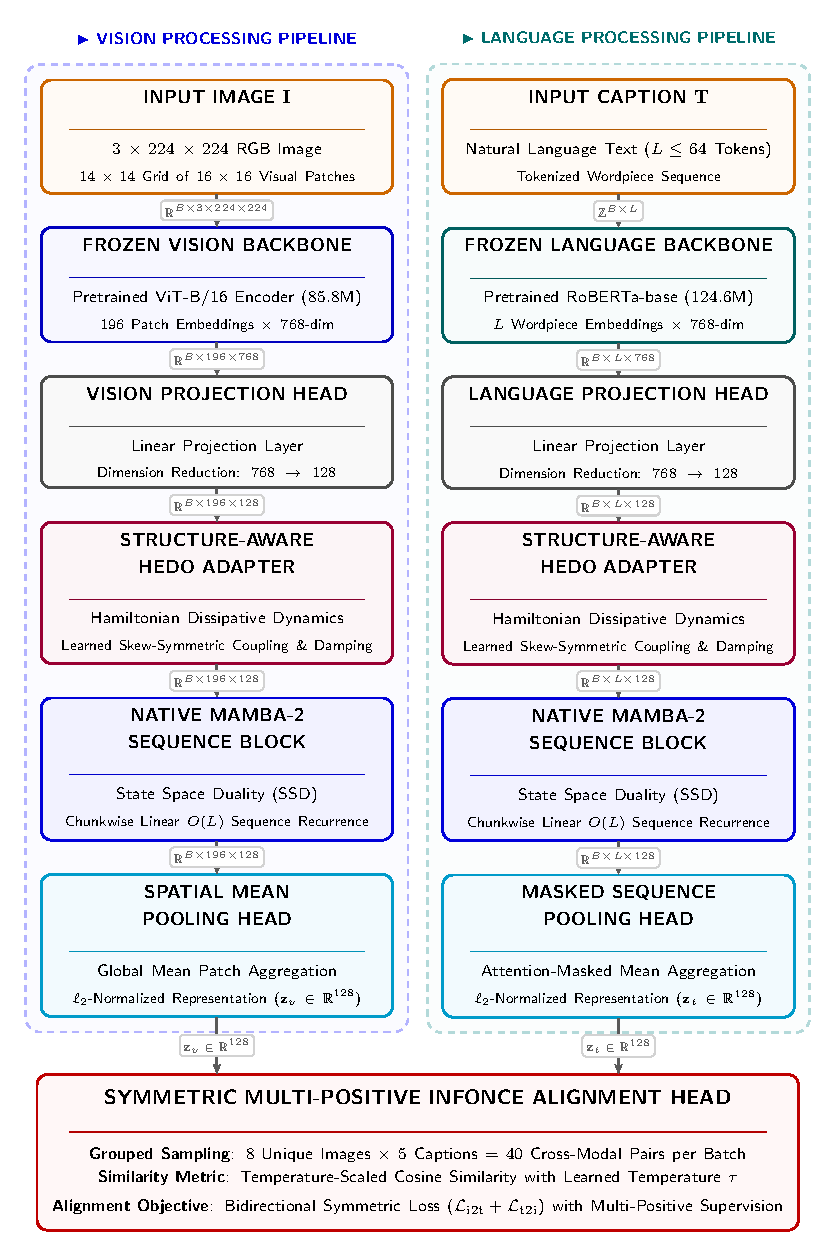
\includegraphics[width=0.78\textwidth]{standalone_architecture.pdf}
\caption{Overall architecture of the proposed Native Mamba-2 cross-modal framework with structure-aware Hamiltonian dissipative adaptation (HEDO). Frozen visual patch features $\mathbf{X}_v$ and language wordpiece features $\mathbf{X}_t$ are linearly projected to $d=128$, adapted via continuous-state coordinate-momentum dynamics, and processed through Native Mamba-2 State Space Duality (SSD) sequence blocks before isotropic semantic pooling and multi-positive symmetric InfoNCE contrastive alignment.}
\label{fig:architecture}
\end{figure*}

As illustrated in Fig.~\ref{fig:architecture}, both modalities operate in parallel streams from input to the contrastive head. For an input image $\mathbf{I}$ and caption $\mathbf{T}$, frozen backbones extract token sequences that are linearly projected to $d=128$. The projected representations are processed by the HEDO adapter and Native Mamba-2 sequence block before modality-specific pooling produces normalized embeddings $\mathbf{z}_v, \mathbf{z}_t \in \mathbb{S}^{127}$ for symmetric multi-positive InfoNCE alignment:
\begin{align}
\mathbf{I} &\to \mathrm{ViT} \to \mathbf{W}_v \to \mathrm{HEDO} \to \mathrm{SSD} \to \mathbf{z}_v \in \mathbb{S}^{127}, \\
\mathbf{T} &\to \mathrm{RoBERTa} \to \mathbf{W}_t \to \mathrm{HEDO} \to \mathrm{SSD} \to \mathbf{z}_t \in \mathbb{S}^{127}.
\end{align}

\subsection{Frozen Vision and Language Encoders}
The visual stream uses $\mathrm{ViT\text{-}B/16}$ ($85.8\text{M}$ parameters) yielding $\mathbf{X}_v \in \mathbb{R}^{B \times 196 \times 768}$, and the language stream uses $\mathrm{RoBERTa\text{-}base}$ ($124.6\text{M}$ parameters) yielding $\mathbf{X}_t \in \mathbb{R}^{B \times L \times 768}$, both kept strictly frozen as formalized in \eqref{eq:frozen_vision}--\eqref{eq:frozen_lang}.

\subsection{Linear Projection}
Both modalities are projected into a common latent dimension $d=128$:
\begin{equation}
\label{eq:projection}
\mathbf{H}_v^{(0)} = \mathbf{X}_v \mathbf{W}_v, \quad \mathbf{H}_t^{(0)} = \mathbf{X}_t \mathbf{W}_t,
\end{equation}
where $\mathbf{W}_v, \mathbf{W}_t \in \mathbb{R}^{768 \times 128}$ are trainable linear projection weight matrices initialized via Xavier uniform initialization. This linear projection reduces the channel dimensionality from 768 to 128, establishing the common working dimension for subsequent adapters and sequence models.

\subsection{Structure-Aware Hamiltonian Dissipative Adapter (HEDO)}
The HEDO adapter introduces a continuous-state inductive bias rooted in dissipative Hamiltonian dynamics.

\subsubsection{Coordinate-Momentum Representation}
For an input sequence representation $\mathbf{x} \in \mathbb{R}^d$ at any token position, canonical coordinates $\mathbf{q} \in \mathbb{R}^d$ and conjugate momenta $\mathbf{p} \in \mathbb{R}^d$ are defined by:
\begin{equation}
\label{eq:hedo_qp}
\mathbf{q} = \mathbf{W}_q \mathbf{x}, \quad \mathbf{p} = \mathbf{W}_p \mathbf{x},
\end{equation}
where $\mathbf{W}_q, \mathbf{W}_p \in \mathbb{R}^{d \times d}$ project the latent token into conjugate phase space coordinates.

\subsubsection{Hamiltonian Energy}
We define the quadratic Hamiltonian energy function:
\begin{equation}
\label{eq:hamiltonian}
\mathcal{H}(\mathbf{q}, \mathbf{p}) = \frac{1}{2} \left( \|\mathbf{q}\|_2^2 + \|\mathbf{p}\|_2^2 \right),
\end{equation}
representing the sum of generalized potential energy $\frac{1}{2}\|\mathbf{q}\|_2^2$ and kinetic energy $\frac{1}{2}\|\mathbf{p}\|_2^2$.

\subsubsection{Skew-Symmetric Interaction}
To parameterize conservative internal interactions while avoiding unbounded growth, we construct an exact skew-symmetric interaction matrix $\mathbf{J} \in \mathbb{R}^{d \times d}$:
\begin{equation}
\label{eq:skew_symmetric}
\mathbf{J} = \frac{\mathbf{A} - \mathbf{A}^T}{\sqrt{d}}, \quad \mathbf{A} \in \mathbb{R}^{d \times d},
\end{equation}
where $\mathbf{A}$ is initialized from $\mathcal{N}(0, 0.01^2)$. By construction, $\mathbf{J}^T = -\mathbf{J}$. For any vector $\mathbf{v}$, the quadratic form vanishes identically ($\mathbf{v}^T \mathbf{J} \mathbf{v} = 0$), ensuring that $\mathbf{J}$ performs purely conservative, norm-preserving rotations in the latent space.

\subsubsection{Dissipative Damping}
Dissipation is enforced via a diagonal positive semi-definite damping matrix $\mathbf{R} \in \mathbb{R}^{d \times d}$:
\begin{equation}
\label{eq:damping_matrix}
\mathbf{R} = \mathrm{diag}\left( 0.05 + 0.95 \cdot \sigma(\boldsymbol{\gamma}) \right), \quad \boldsymbol{\gamma} \in \mathbb{R}^d,
\end{equation}
where $\sigma(\cdot)$ denotes the sigmoid function, ensuring each diagonal entry is strictly bounded in $[0.05, 1.0]$. The strictly positive floor $0.05$ guarantees non-zero energy dissipation.

\subsubsection{Continuous-Time Dynamics}
The continuous-time equations of motion coupling coordinates and momenta are governed by:
\begin{equation}
\label{eq:hedo_ode}
\begin{aligned}
\begin{bmatrix} \dot{\mathbf{q}} \\ \dot{\mathbf{p}} \end{bmatrix} 
&= \begin{bmatrix} \mathbf{0} & \mathbf{I} \\ -\mathbf{I} & -\mathbf{R} \end{bmatrix} 
\begin{bmatrix} \nabla_{\mathbf{q}}\mathcal{H} \\ \nabla_{\mathbf{p}}\mathcal{H} \end{bmatrix} 
+ \begin{bmatrix} \mathbf{q} \mathbf{J}^T \\ \mathbf{p} \mathbf{J}^T \end{bmatrix} \\
&= \begin{bmatrix} \mathbf{p} + \mathbf{q} \mathbf{J}^T \\ -\mathbf{q} + \mathbf{p} \mathbf{J}^T - \mathbf{R} \odot \mathbf{p} \end{bmatrix}.
\end{aligned}
\end{equation}
This formulation represents a port-Hamiltonian system with internal dissipation $\mathbf{R}$ and learned symplectic rotation $\mathbf{J}$.

\subsubsection{Energy-Boundedness Proposition}
\begin{proposition}[Energy Boundedness in Continuous HEDO]
Under the unforced dynamics of \eqref{eq:hedo_ode}, the time derivative of the Hamiltonian $\mathcal{H}(\mathbf{q}, \mathbf{p})$ satisfies:
\begin{equation}
\frac{d}{dt}\mathcal{H}(\mathbf{q}, \mathbf{p}) = -\mathbf{p}^T \mathbf{R} \mathbf{p} \le -0.05 \|\mathbf{p}\|_2^2 \le 0.
\end{equation}
\end{proposition}
\begin{proof}
By the chain rule:
\begin{align}
\frac{d}{dt}\mathcal{H} &= \mathbf{q}^T \dot{\mathbf{q}} + \mathbf{p}^T \dot{\mathbf{p}} \nonumber \\
&= \mathbf{q}^T (\mathbf{p} + \mathbf{q} \mathbf{J}^T) + \mathbf{p}^T (-\mathbf{q} + \mathbf{p} \mathbf{J}^T - \mathbf{R} \mathbf{p}) \nonumber \\
&= \mathbf{q}^T \mathbf{p} + \mathbf{q}^T \mathbf{J}^T \mathbf{q} - \mathbf{p}^T \mathbf{q} + \mathbf{p}^T \mathbf{J}^T \mathbf{p} - \mathbf{p}^T \mathbf{R} \mathbf{p}.
\end{align}
Since $\mathbf{J}$ is skew-symmetric, for any vector $\mathbf{v}$, $\mathbf{v}^T \mathbf{J}^T \mathbf{v} = -\mathbf{v}^T \mathbf{J} \mathbf{v} = 0$. Furthermore, $\mathbf{q}^T \mathbf{p} - \mathbf{p}^T \mathbf{q} = 0$. Thus:
\begin{equation}
\frac{d}{dt}\mathcal{H} = -\mathbf{p}^T \mathbf{R} \mathbf{p}.
\end{equation}
Since $\mathbf{R}_{i,i} \ge 0.05 > 0$, $\frac{d}{dt}\mathcal{H} \le 0$, proving that energy is monotonically non-increasing.
\end{proof}

\subsubsection{Bounded Discrete Integration}
To integrate the continuous ODE in discrete time without numerical instability, we employ a bounded Euler step $\Delta t = 0.05 + 0.10 \cdot \sigma(\tau_{\Delta t}) \in [0.05, 0.15]$:
\begin{equation}
\label{eq:euler_step}
\mathbf{q}_{\mathrm{new}} = \mathbf{q} + \Delta t \cdot \dot{\mathbf{q}}, \quad \mathbf{p}_{\mathrm{new}} = \mathbf{p} + \Delta t \cdot \dot{\mathbf{p}}.
\end{equation}

\subsubsection{Residual Update}
The updated canonical variables are combined and normalized, producing a residual update:
\begin{equation}
\label{eq:hedo_out}
\mathbf{x}_{\mathrm{out}} = \mathbf{x} + 0.10 \cdot \mathbf{W}_o \mathrm{LayerNorm}(\mathbf{q}_{\mathrm{new}} + \mathbf{p}_{\mathrm{new}}),
\end{equation}
where $\mathbf{W}_o \in \mathbb{R}^{d \times d}$ is initialized via Xavier uniform with gain $0.5$. The $0.10$ scaling ensures the adapter acts as a near-identity mapping at initialization.

\subsection{Native Mamba-2 Sequence Processing}
Following HEDO, sequences are processed through official Native Mamba-2 sequence blocks~\cite{dao2024transformers}. The block configuration is parameterized by:
\begin{equation}
\label{eq:mamba2_params}
d_{\mathrm{model}} = 128, \quad d_{\mathrm{state}} = 64, \quad d_{\mathrm{conv}} = 4, \quad \mathrm{expand} = 2,
\end{equation}
with head dimension $64$ and chunk size $Q = 16$. 

Given an input sequence $\mathbf{H} \in \mathbb{R}^{B \times L \times 128}$, the input is first expanded to dimension $E \cdot d = 256$, processed by a 1D depthwise convolution of kernel size $4$, and projected into input-dependent SSM parameters. Within each chunk of length $Q$, SSD computes the inter-chunk recurrence and intra-chunk semi-separable transformations via tensor cores, producing transformed representations $\mathbf{Y} \in \mathbb{R}^{B \times L \times 128}$.

\subsection{Multi-Scale State Aggregation (MSA)}
In standard Mamba-2 alignment, sequence pooling is performed via masked mean pooling:
\begin{equation}
\label{eq:global_mean}
\bar{\mathbf{y}}_{\mathrm{global}} = \frac{\sum_{i=1}^L m_i \mathbf{Y}_i}{\sum_{i=1}^L m_i},
\end{equation}
where $m_i \in \{0, 1\}$ denotes token validity.

The MSA module tests whether incorporating multi-resolution temporal features improves alignment. For chunk size $Q=16$, chunk boundary indices $c_k = \min(k \cdot Q, L) - 1$ are collected to extract boundary states $\mathbf{Y}_{\mathrm{boundary}} \in \mathbb{R}^{B \times K \times d}$, where $K = \lceil L / Q \rceil$. The boundary states are mean-pooled:
\begin{equation}
\label{eq:boundary_mean}
\bar{\mathbf{y}}_{\mathrm{boundary}} = \frac{1}{K}\sum_{k=1}^K \mathbf{Y}_{\mathrm{boundary}, k}.
\end{equation}
Additionally, the terminal valid recurrent token is extracted:
\begin{equation}
\label{eq:terminal_state}
\mathbf{y}_{\mathrm{last}} = \mathbf{Y}_{B, L_{\mathrm{valid}}-1}.
\end{equation}
The multi-scale fusion combines all three representations:
\begin{equation}
\label{eq:msa_fusion}
\mathbf{y}_{\mathrm{fused}} = \mathbf{W}_{\mathrm{proj}} \mathrm{LayerNorm}\left( [\bar{\mathbf{y}}_{\mathrm{global}} \,\|\, \bar{\mathbf{y}}_{\mathrm{boundary}} \,\|\, \mathbf{y}_{\mathrm{last}}] \right),
\end{equation}
where $\mathbf{W}_{\mathrm{proj}} \in \mathbb{R}^{3d \times d}$.

\subsection{Adaptive Variational State Coupling (AVSC)}
AVSC evaluates intermediate latent regularized coupling between image and text streams during training. Pooled boundary representations $\mathbf{h}_v, \mathbf{h}_t \in \mathbb{R}^d$ are mapped to diagonal Gaussian posteriors:
\begin{align}
\label{eq:avsc_params_v}
\boldsymbol{\mu}_v = \mathbf{W}_{\mu, v} \mathbf{h}_v, \quad \log \boldsymbol{\sigma}_v^2 = \mathrm{clamp}(\mathbf{W}_{\sigma, v} \mathbf{h}_v, -6.0, 2.0), \\
\label{eq:avsc_params_t}
\boldsymbol{\mu}_t = \mathbf{W}_{\mu, t} \mathbf{h}_t, \quad \log \boldsymbol{\sigma}_t^2 = \mathrm{clamp}(\mathbf{W}_{\sigma, t} \mathbf{h}_t, -6.0, 2.0).
\end{align}
The symmetric Kullback-Leibler divergence between $q_v = \mathcal{N}(\boldsymbol{\mu}_v, \boldsymbol{\Sigma}_v)$ and $q_t = \mathcal{N}(\boldsymbol{\mu}_t, \boldsymbol{\Sigma}_t)$ is:
\begin{equation}
\label{eq:kl_sym}
\mathcal{D}_{\mathrm{KL}}^{\mathrm{sym}}(q_v, q_t) = \frac{1}{2}\left( D_{\mathrm{KL}}(q_v \parallel q_t) + D_{\mathrm{KL}}(q_t \parallel q_v) \right),
\end{equation}
where each component divergence is computed analytically:
\begin{equation}
\label{eq:kl_component}
\begin{aligned}
D_{\mathrm{KL}}(q_v \parallel q_t) = \frac{1}{2} \sum_{k=1}^d \bigg( &\log \frac{\sigma_{t,k}^2}{\sigma_{v,k}^2} \\
&+ \frac{\sigma_{v,k}^2 + (\mu_{v,k} - \mu_{t,k})^2}{\sigma_{t,k}^2} - 1 \bigg).
\end{aligned}
\end{equation}
To prevent catastrophic interference from unaligned pairs, the loss is gated by a detached confidence weight $w_{\mathrm{gate}} \in [0, 1]$ derived from cosine agreement:
\begin{equation}
\label{eq:avsc_loss}
\mathcal{L}_{\mathrm{KL}} = \lambda_{\mathrm{KL}} \cdot \frac{1}{B}\sum_{i=1}^B w_{\mathrm{gate}, i} \cdot \mathcal{D}_{\mathrm{KL}, i}^{\mathrm{sym}},
\end{equation}
where $\lambda_{\mathrm{KL}} = 10^{-3}$. At inference, embeddings remain strictly deterministic and unimodal.

\subsection{Multi-Positive Contrastive Objective}
Cross-modal alignment is supervised via a symmetric multi-positive InfoNCE loss. In Flickr8k, each image corresponds to 5 captions. An atomic grouped batch sampler groups 8 unique images and all 5 corresponding captions per image, yielding a batch of $B_{\mathrm{img}} = 8$ and $B_{\mathrm{txt}} = 40$.

Let $\mathbf{Z}_v \in \mathbb{R}^{8 \times d}$ be the normalized visual embeddings of the 8 unique images, and let $\mathbf{Z}_t \in \mathbb{R}^{40 \times d}$ be the normalized textual embeddings. The cosine similarity matrix $\mathbf{S} \in \mathbb{R}^{8 \times 40}$ is:
\begin{equation}
\label{eq:similarity_matrix}
S_{i, j} = \exp(\tau) \cdot (\mathbf{z}_{v, i} \cdot \mathbf{z}_{t, j}),
\end{equation}
where $\tau$ is a learnable log-temperature parameter initialized to $\log(1/0.07) \approx 2.659$.

For each unique image $i \in \{1, \dots, 8\}$, let $\mathcal{P}(i) \subset \{1, \dots, 40\}$ denote the set of 5 positive caption indices ($|\mathcal{P}(i)| = 5$). The image-to-text loss is:
\begin{equation}
\label{eq:infonce_i2t}
\mathcal{L}_{i2t} = -\frac{1}{8} \sum_{i=1}^8 \frac{1}{|\mathcal{P}(i)|} \sum_{j \in \mathcal{P}(i)} \log \frac{\exp(S_{i, j})}{\sum_{k=1}^{40} \exp(S_{i, k})}.
\end{equation}
Similarly, for each caption $j \in \{1, \dots, 40\}$, let $i^*(j) \in \{1, \dots, 8\}$ denote its unique parent image. The text-to-image loss is:
\begin{equation}
\label{eq:infonce_t2i}
\mathcal{L}_{t2i} = -\frac{1}{40} \sum_{j=1}^{40} \log \frac{\exp(S_{i^*(j), j})}{\sum_{i=1}^{8} \exp(S_{i, j})}.
\end{equation}
The total alignment objective is:
\begin{equation}
\label{eq:total_loss}
\mathcal{L} = \frac{1}{2}\left( \mathcal{L}_{i2t} + \mathcal{L}_{t2i} \right) + \mathcal{L}_{\mathrm{KL}}.
\end{equation}

The end-to-end training procedure for the proposed Native Mamba-2 + HEDO framework is formalized in Algorithm~\ref{alg:training}.

\begin{algorithm}[htbp]
\caption{Training Procedure for Native Mamba-2 + HEDO}
\label{alg:training}
\begin{algorithmic}[1]
\REQUIRE Image-caption dataset $\mathcal{D}$, frozen backbones $\mathrm{ViT\text{-}B/16}$, $\mathrm{RoBERTa\text{-}base}$, epochs $E=10$, batch size $B_{\mathrm{img}}=8, B_{\mathrm{txt}}=40$
\ENSURE Trained projection layers $\mathbf{W}_v, \mathbf{W}_t$, HEDO parameters $\boldsymbol{\theta}_{\mathrm{hedo}}$, Native Mamba-2 parameters $\boldsymbol{\theta}_{\mathrm{ssd}}$, log-temperature $\tau$
\STATE Initialize projection layers $\mathbf{W}_v, \mathbf{W}_t \in \mathbb{R}^{768 \times 128}$, HEDO parameters $\mathbf{W}_q, \mathbf{W}_p, \mathbf{A}, \boldsymbol{\gamma}, \mathbf{W}_o$, Mamba-2 SSD weights, and $\tau \leftarrow \log(1/0.07)$
\FOR{epoch $= 1$ \TO $E$}
    \FOR{each grouped batch $(\mathcal{B}_{\mathrm{img}}, \mathcal{B}_{\mathrm{txt}}) \sim \mathcal{D}$}
        \STATE Extract frozen visual patch features $\mathbf{X}_v \leftarrow \mathrm{ViT}(\mathcal{B}_{\mathrm{img}}) \in \mathbb{R}^{8 \times 196 \times 768}$
        \STATE Extract frozen text token features $\mathbf{X}_t \leftarrow \mathrm{RoBERTa}(\mathcal{B}_{\mathrm{txt}}) \in \mathbb{R}^{40 \times L \times 768}$
        \STATE Project to latent dimension: $\mathbf{H}_v^{(0)} \leftarrow \mathbf{X}_v \mathbf{W}_v$, $\mathbf{H}_t^{(0)} \leftarrow \mathbf{X}_t \mathbf{W}_t \in \mathbb{R}^{\cdot \times \cdot \times 128}$
        \STATE Apply HEDO adapter: $\mathbf{H}_v \leftarrow \mathrm{HEDO}(\mathbf{H}_v^{(0)})$, $\mathbf{H}_t \leftarrow \mathrm{HEDO}(\mathbf{H}_t^{(0)})$ via \eqref{eq:hedo_out}
        \STATE Process through Native Mamba-2 SSD blocks: $\mathbf{Y}_v \leftarrow \mathrm{SSD}_v(\mathbf{H}_v)$, $\mathbf{Y}_t \leftarrow \mathrm{SSD}_t(\mathbf{H}_t)$
        \STATE Compute masked global mean pooling and $\ell_2$-normalization: $\mathbf{z}_v \leftarrow \mathrm{Pool}(\mathbf{Y}_v)$, $\mathbf{z}_t \leftarrow \mathrm{Pool}(\mathbf{Y}_t) \in \mathbb{S}^{127}$
        \STATE Compute cosine similarity matrix: $\mathbf{S} \leftarrow \exp(\tau) \cdot (\mathbf{z}_v \mathbf{z}_t^T) \in \mathbb{R}^{8 \times 40}$
        \STATE Compute symmetric multi-positive InfoNCE loss: $\mathcal{L}_{\mathrm{NCE}} \leftarrow \frac{1}{2}(\mathcal{L}_{i2t} + \mathcal{L}_{t2i})$ via \eqref{eq:infonce_i2t}--\eqref{eq:infonce_t2i}
        \IF{AVSC enabled}
            \STATE Compute confidence-gated symmetric KL divergence $\mathcal{L}_{\mathrm{KL}}$ via \eqref{eq:kl_component}
            \STATE Total objective: $\mathcal{L} \leftarrow \mathcal{L}_{\mathrm{NCE}} + \mathcal{L}_{\mathrm{KL}}$
        \ELSE
            \STATE Total objective: $\mathcal{L} \leftarrow \mathcal{L}_{\mathrm{NCE}}$
        \ENDIF
        \STATE Backpropagate gradients $\nabla_{\boldsymbol{\theta}} \mathcal{L}$
        \STATE Clip gradients: $\mathbf{g} \leftarrow \mathrm{clip}(\mathbf{g}, \|\mathbf{g}\|_2 \le 1.0)$
        \STATE Update trainable parameters $\boldsymbol{\theta}$ using AdamW ($\eta = 10^{-4}$, weight decay $10^{-4}$)
    \ENDFOR
\ENDFOR
\RETURN Trained model parameters $\{\mathbf{W}_v, \mathbf{W}_t, \boldsymbol{\theta}_{\mathrm{hedo}}, \boldsymbol{\theta}_{\mathrm{ssd}}, \tau\}$
\end{algorithmic}
\end{algorithm}

% =========================================================================
% SECTION V: EXPERIMENTAL METHODOLOGY
% =========================================================================
\section{Experimental Methodology}
\label{sec:methodology}

\subsection{Dataset}
We evaluate on the canonical Flickr8k dataset~\cite{hodosh2013framing}, comprising 8,000 images, each paired with 5 human-written captions (6,000 training, 1,000 validation, and 1,000 test images).

\subsection{Data Preprocessing}
Images are resized to $224 \times 224$ and normalized using ImageNet statistics. Text is tokenized using the standard RoBERTa tokenizer with maximum sequence length truncated to 64 tokens.

\subsection{Training Configuration}
All models are trained for 10 epochs using AdamW with an initial learning rate of $\eta = 10^{-4}$ and weight decay $10^{-4}$. Batch size is fixed to 8 unique images and 40 captions per iteration. Gradient clipping is enforced at a maximum $\ell_2$ norm of $1.0$.

\subsection{Experimental Configurations}
To systematically decouple the individual and joint effects of HEDO, Mamba-2, MSA, and AVSC, we evaluate a controlled 8-configuration ablation matrix, summarized in Table~\ref{tab:configurations}.

\begin{table}[htbp]
\centering
\caption{Ablation Configuration Matrix Defining Architectural Variants.}
\label{tab:configurations}
\begin{tabular}{lcccc}
\toprule
\textbf{Configuration ID} & \textbf{HEDO} & \textbf{Mamba-2} & \textbf{MSA} & \textbf{AVSC} \\
\midrule
\texttt{baseline} & $\times$ & $\times$ & $\times$ & $\times$ \\
\texttt{mamba2\_hedo\_v2} & $\checkmark$ & $\checkmark$ & $\times$ & $\times$ \\
\texttt{mamba2\_msa\_v2} & $\times$ & $\checkmark$ & $\checkmark$ & $\times$ \\
\texttt{hedo\_msa\_v2} & $\checkmark$ & $\times$ & $\checkmark$ & $\times$ \\
\texttt{avsc\_msa\_v2} & $\times$ & $\times$ & $\checkmark$ & $\checkmark$ \\
\texttt{mamba2\_avsc\_v2} & $\times$ & $\checkmark$ & $\times$ & $\checkmark$ \\
\texttt{full\_v2} (All) & $\checkmark$ & $\checkmark$ & $\checkmark$ & $\checkmark$ \\
\texttt{hedo\_avsc\_v2} & $\checkmark$ & $\times$ & $\times$ & $\checkmark$ \\
\bottomrule
\end{tabular}
\end{table}

Table~\ref{tab:configurations} defines the 8-configuration ablation matrix designed to isolate the individual and joint effects of HEDO, Mamba-2, MSA, and AVSC across the eight evaluated models. Full V2 activates all four mechanisms simultaneously and is included as a compositional stress test rather than as an assumption that all components are individually beneficial.

\subsection{Evaluation Metrics}
Retrieval performance is evaluated on the standard 1,000-image test set ($1,000$ images $\times$ $5,000$ captions):
\begin{itemize}
    \item \textbf{Image-to-Text (i2t) Retrieval}: Recall@1, Recall@5, Recall@10, and Median Rank (MedR).
    \item \textbf{Text-to-Image (t2i) Retrieval}: Recall@1, Recall@5, Recall@10, and Median Rank (MedR).
    \item \textbf{Mean Recall (MR)}: The primary arithmetic mean across all six recall metrics:
    \begin{equation}
    \label{eq:mean_recall}
    \begin{aligned}
    \mathrm{MR} = \frac{1}{6} \Big( &\mathrm{R@1}_{i2t} + \mathrm{R@5}_{i2t} + \mathrm{R@10}_{i2t} \\
    &+ \mathrm{R@1}_{t2i} + \mathrm{R@5}_{t2i} + \mathrm{R@10}_{t2i} \Big).
    \end{aligned}
    \end{equation}
\end{itemize}

\subsection{Statistical Evaluation Protocol}
For every configuration $c \in \{1, \dots, 7\}$, we compute the paired delta relative to the baseline across identical seeds $s \in \{42, 43, 44\}$:
\begin{equation}
\label{eq:paired_delta}
\Delta_{c, s} = \mathrm{MR}_{c, s} - \mathrm{MR}_{\mathrm{baseline}, s}.
\end{equation}
We report the sample mean $\bar{\Delta}_c$, sample standard deviation $s_c$, and two-tailed 95\% Student-$t$ confidence intervals:
\begin{equation}
\label{eq:confidence_interval}
\mathrm{CI}_{95\%} = \left[ \bar{\Delta}_c - t_{0.025, 2} \frac{s_c}{\sqrt{3}}, \; \bar{\Delta}_c + t_{0.025, 2} \frac{s_c}{\sqrt{3}} \right],
\end{equation}
where $t_{0.025, 2} = 4.303$. A hypothesis of improvement is classified as:
\begin{itemize}
    \item \textbf{SUPPORTED}: $\bar{\Delta}_c > 0$ and $\mathrm{CI}_{95\%}$ strictly excludes zero ($\mathrm{CI}_{\mathrm{low}} > 0$).
    \item \textbf{NOT SUPPORTED (NO STAT. DIFF.)}: The null hypothesis of zero difference cannot be rejected as $\mathrm{CI}_{95\%}$ contains zero ($\mathrm{CI}_{\mathrm{low}} \le 0 \le \mathrm{CI}_{\mathrm{high}}$).
    \item \textbf{CONTRADICTED}: $\bar{\Delta}_c < 0$ and $\mathrm{CI}_{95\%}$ strictly excludes zero ($\mathrm{CI}_{\mathrm{high}} < 0$).
\end{itemize}

\subsection{Reproducibility and Audit Controls}
To guarantee numerical reproducibility and prevent silent execution failures, the training harness incorporates strict hardware and numerical assertion gates:
\begin{itemize}
    \item \textbf{Finite Tensor Monitor}: Every forward and backward pass asserts $\mathrm{isfinite}(\mathbf{T})$ across all intermediate activations, logit matrices, and gradient tensors.
    \item \textbf{Native Mamba-2 Verification}: Direct inspection confirms loading of official \texttt{mamba\_ssm.modules.mamba2.Mamba2} GPU CUDA kernels.
    \item \textbf{Three-Seed Replication}: Every configuration is executed independently across seeds $42, 43, 44$, generating 24 fully audited training runs. The methodology hash is recorded as \texttt{1753cfb7...1af54}\footnote{Full 64-character SHA-256 methodology hash: \texttt{1753cfb7181e6355cd79bd6dd9a3ceb6}\allowbreak\texttt{26b4de36f8dbcfe0807591b89cd1af54}.}.
\end{itemize}

The complete multi-seed experimental audit protocol is formalized in Algorithm~\ref{alg:audit}.

\begin{algorithm}[htbp]
\caption{Multi-Seed Experimental Audit Protocol}
\label{alg:audit}
\begin{algorithmic}[1]
\REQUIRE Configuration set $\mathcal{C} = \{c_0, c_1, \dots, c_7\}$, seeds $\mathcal{S} = \{42, 43, 44\}$, test dataset $\mathcal{D}_{\mathrm{test}}$
\ENSURE Paired deltas $\bar{\Delta}_c$, 95\% confidence intervals $\mathrm{CI}_{95\%}$, pre-registered verdicts
\FOR{each configuration $c \in \mathcal{C}$}
    \FOR{each random seed $s \in \mathcal{S}$}
        \STATE Set random seed $s$ across PyTorch, NumPy, Python runtime
        \STATE Assert GPU execution environment and official Mamba-2 CUDA kernel loading
        \STATE Train model configuration $c$ using Algorithm~\ref{alg:training} with finite tensor monitoring
        \STATE Evaluate test retrieval on $\mathcal{D}_{\mathrm{test}}$: compute $\mathrm{R@1}, \mathrm{R@5}, \mathrm{R@10}, \mathrm{MedR}$ for i2t and t2i
        \STATE Compute Mean Recall: $\mathrm{MR}_{c, s} \leftarrow \frac{1}{6}\sum \mathrm{Recall}$ via \eqref{eq:mean_recall}
        \STATE Measure head/end-to-end latency, throughput, and peak VRAM
    \ENDFOR
    \STATE Compute aggregate metrics: $\mu_c \leftarrow \mathrm{mean}_s(\mathrm{MR}_{c, s})$, $\sigma_c \leftarrow \mathrm{std}_s(\mathrm{MR}_{c, s})$
    \IF{$c \ne \mathrm{baseline}$}
        \STATE Compute per-seed paired deltas: $\Delta_{c, s} \leftarrow \mathrm{MR}_{c, s} - \mathrm{MR}_{\mathrm{baseline}, s}$ via \eqref{eq:paired_delta}
        \STATE Compute sample mean $\bar{\Delta}_c$ and sample standard deviation $s_c$
        \STATE Compute 95\% Student-$t$ confidence interval: $\mathrm{CI}_{95\%} \leftarrow [\bar{\Delta}_c \pm t_{0.025, 2} \frac{s_c}{\sqrt{3}}]$ via \eqref{eq:confidence_interval}
        \IF{$\mathrm{CI}_{95\%} \subset (0, \infty)$}
            \STATE Set Verdict $\leftarrow$ \textbf{SUPPORTED}
        \ELSIF{$0 \in \mathrm{CI}_{95\%}$}
            \STATE Set Verdict $\leftarrow$ \textbf{NO STAT. DIFF.}
        \ELSE
            \STATE Set Verdict $\leftarrow$ \textbf{CONTRADICTED}
        \ENDIF
    \ENDIF
\ENDFOR
\STATE Generate tabular summaries (Tables~\ref{tab:ablation_results}, \ref{tab:paired_deltas}, \ref{tab:efficiency_results}) and statistical figures (Figs.~\ref{fig:factorial_recall}--\ref{fig:seed_stability_metrics})
\RETURN Audited benchmark results and statistical decisions
\end{algorithmic}
\end{algorithm}

% =========================================================================
% SECTION VI: RESULTS
% =========================================================================
\section{Results}
\label{sec:results}

\subsection{Overall Retrieval Performance}
The empirical retrieval metrics across all 8 configurations are compiled in Table~\ref{tab:ablation_results} and illustrated across recall thresholds in Fig.~\ref{fig:factorial_recall}. 

\begin{table*}[!t]
\centering
\caption{Complete Ablation Retrieval Performance on Flickr8k Across 8 Configurations (Mean $\pm$ Standard Deviation across 3 Seeds, $N=24$).}
\label{tab:ablation_results}
\resizebox{\textwidth}{!}{%
\begin{tabular}{lcccccccccc}
\toprule
\textbf{Configuration} & \textbf{i2t R@1 (\%)} & \textbf{i2t R@5 (\%)} & \textbf{i2t R@10 (\%)} & \textbf{t2i R@1 (\%)} & \textbf{t2i R@5 (\%)} & \textbf{t2i R@10 (\%)} & \textbf{Mean Recall (\%)} & \textbf{i2t MedR} & \textbf{t2i MedR} & \textbf{Verdict} \\
\midrule
\textbf{Baseline} & $16.53 \pm 0.70$ & $43.27 \pm 0.72$ & $57.47 \pm 1.14$ & $13.92 \pm 0.45$ & $38.31 \pm 0.38$ & $53.45 \pm 0.49$ & $37.16 \pm 0.57$ & $7.67 \pm 0.58$ & $9.00 \pm 0.00$ & \textit{Reference} \\
\textbf{Mamba-2 + HEDO} & $\mathbf{17.40 \pm 0.62}$ & $\mathbf{43.47 \pm 1.85}$ & $57.20 \pm 1.10$ & $\mathbf{14.20 \pm 0.58}$ & $38.25 \pm 0.47$ & $53.35 \pm 0.50$ & $\mathbf{37.31 \pm 0.68}$ & $\mathbf{7.67 \pm 0.58}$ & $\mathbf{9.00 \pm 0.00}$ & \textbf{No Stat. Diff.} \\
\midrule
\textbf{Mamba-2 + MSA} & $9.77 \pm 0.51$ & $29.53 \pm 0.95$ & $42.90 \pm 1.04$ & $8.92 \pm 0.47$ & $28.22 \pm 0.59$ & $41.98 \pm 0.75$ & $26.89 \pm 0.68$ & $13.83 \pm 0.76$ & $14.67 \pm 0.58$ & Contradicted \\
\textbf{HEDO + MSA} & $9.47 \pm 0.47$ & $29.50 \pm 1.47$ & $42.87 \pm 1.59$ & $8.33 \pm 0.42$ & $27.45 \pm 0.09$ & $40.84 \pm 0.84$ & $26.41 \pm 0.49$ & $14.67 \pm 0.58$ & $15.33 \pm 0.58$ & Contradicted \\
\midrule
\textbf{AVSC + MSA} & $1.47 \pm 0.32$ & $6.40 \pm 1.87$ & $11.50 \pm 1.84$ & $1.50 \pm 0.26$ & $6.51 \pm 0.28$ & $12.48 \pm 0.76$ & $6.64 \pm 0.82$ & $81.67 \pm 5.84$ & $61.33 \pm 2.89$ & Contradicted \\
\textbf{Mamba-2 + AVSC} & $1.80 \pm 0.78$ & $6.27 \pm 1.10$ & $11.87 \pm 0.96$ & $1.05 \pm 0.32$ & $5.55 \pm 1.38$ & $10.19 \pm 2.74$ & $6.12 \pm 1.14$ & $99.83 \pm 21.50$ & $72.33 \pm 14.74$ & Contradicted \\
\textbf{Full V2 (All)} & $1.47 \pm 0.31$ & $5.97 \pm 0.47$ & $10.73 \pm 0.68$ & $1.25 \pm 0.29$ & $5.60 \pm 0.69$ & $10.69 \pm 1.09$ & $5.95 \pm 0.42$ & $94.33 \pm 6.66$ & $69.67 \pm 3.79$ & Contradicted \\
\textbf{HEDO + AVSC} & $1.03 \pm 0.12$ & $4.93 \pm 0.90$ & $9.27 \pm 1.05$ & $1.01 \pm 0.23$ & $4.83 \pm 1.15$ & $9.20 \pm 1.89$ & $5.04 \pm 0.84$ & $103.17 \pm 10.13$ & $79.00 \pm 13.23$ & Contradicted \\
\bottomrule
\end{tabular}%
}
\end{table*}

\begin{figure*}[!t]
\centering
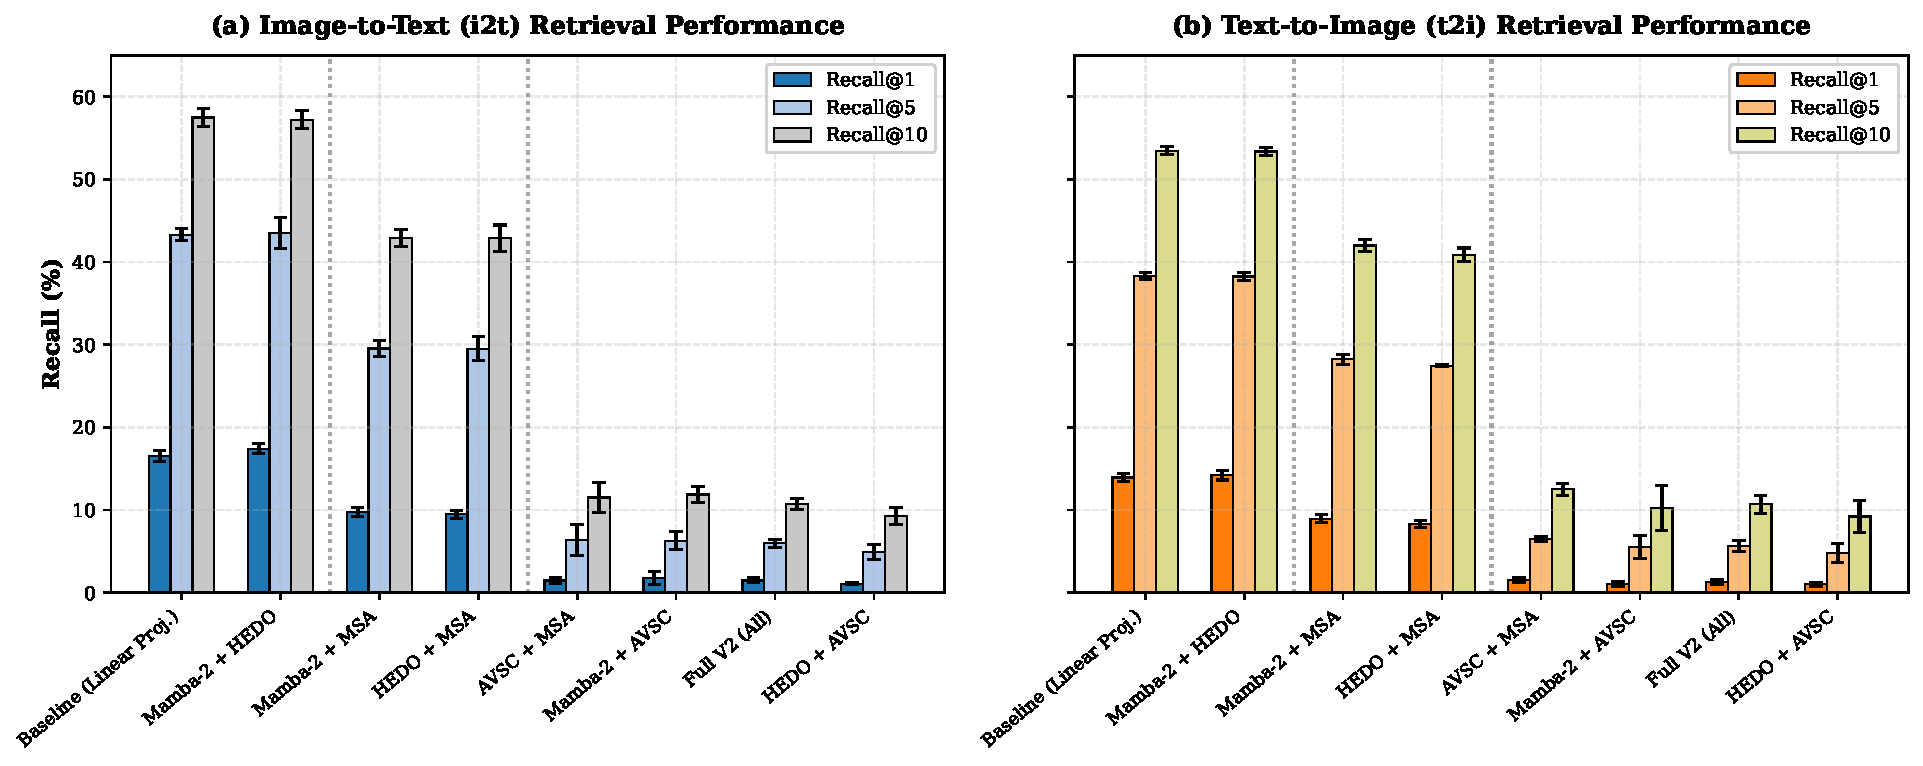
\includegraphics[width=0.96\textwidth]{fig_factorial_recall.pdf}
\caption{Controlled ablation benchmark on Flickr8k across all 8 configurations (3 independent random seeds, $N=24$ runs). (a) Image-to-Text (i2t) Recall@1, Recall@5, and Recall@10. (b) Text-to-Image (t2i) Recall@1, Recall@5, and Recall@10. Error bars denote $\pm 1$ standard deviation. Note the striking bifurcation between the stable regime with no detected difference from baseline (Baseline and Mamba-2 + HEDO) and the severe degradation regimes (MSA and AVSC).}
\label{fig:factorial_recall}
\end{figure*}

As reported in Table~\ref{tab:ablation_results}, the baseline model achieves a Mean Recall of $37.16 \pm 0.57\%$, with Image-to-Text (i2t) R@1 of $16.53\%$ and Text-to-Image (t2i) R@1 of $13.92\%$. Across the eight configurations, performance bifurcates cleanly into two distinct regimes: a stable regime where performance is statistically indistinguishable from baseline (Baseline and Mamba-2 + HEDO) and severe degradation regimes (MSA and AVSC). As visually evident in Fig.~\ref{fig:factorial_recall}, this bifurcation is uniform across all recall thresholds.

\subsection{HEDO + Native Mamba-2 Evaluation}
Equipping the architecture with the Hamiltonian-inspired dissipative adapter and Native Mamba-2 sequence blocks (\texttt{mamba2\_hedo\_v2}) yields a Mean Recall of $37.31 \pm 0.68\%$, with i2t R@1 reaching $17.40 \pm 0.62\%$ and t2i R@1 reaching $14.20 \pm 0.58\%$. As shown in Table~\ref{tab:paired_deltas}, the mean paired delta is $+0.1533$ pp, with a 95\% confidence interval of $[-1.4246, +1.7313]$ pp ($n=3$ paired runs). Because the confidence interval encompasses zero, the hypothesis of a statistically significant improvement ($H_1$) is classified as \textbf{NOT SUPPORTED} (no statistically significant difference was detected under the present three-seed evaluation). 

These results indicate that Native Mamba-2 combined with the HEDO dissipative adapter preserves baseline-level retrieval performance under the evaluated conditions, without observed numerical instability, while maintaining low computational overhead.

\subsection{MSA Ablation Analysis}
Configurations incorporating Multi-Scale State Aggregation (\texttt{mamba2\_msa\_v2} and \texttt{hedo\_msa\_v2}) exhibit a sharp and consistent drop in retrieval capability. \texttt{mamba2\_msa\_v2} attains a Mean Recall of $26.89 \pm 0.68\%$, representing a severe paired delta of $-10.2711$ pp (95\% CI: $[-13.1018, -7.4404]$ pp). Similarly, \texttt{hedo\_msa\_v2} achieves $26.41 \pm 0.49\%$ ($\Delta = -10.7489$ pp, 95\% CI: $[-12.3816, -9.1161]$ pp). Both results strictly exclude zero and contradict Hypothesis 2 ($H_2$). Instead of enriching sequence representations, multi-scale chunk boundary and terminal token states substantially degrade retrieval quality.

\subsection{AVSC Ablation Analysis}
The most striking empirical outcome is that Adaptive Variational State Coupling is associated with severe alignment degradation. Across all four configurations containing AVSC (\texttt{avsc\_msa\_v2}, \texttt{mamba2\_avsc\_v2}, \texttt{full\_v2}, and \texttt{hedo\_avsc\_v2}), Mean Recall drops precipitously to $5.04\%-6.64\%$, consistent with dimensional collapse under the evaluated formulation. 

The paired deltas are uniformly severe:
\begin{itemize}
    \item \textbf{AVSC + MSA}: $\Delta = -30.52$ pp (95\% CI: $[-32.49, -28.54]$ pp)
    \item \textbf{Mamba-2 + AVSC}: $\Delta = -31.04$ pp (95\% CI: $[-35.26, -26.81]$ pp)
    \item \textbf{Full V2 (All)}: $\Delta = -31.21$ pp (95\% CI: $[-32.60, -29.81]$ pp)
    \item \textbf{HEDO + AVSC}: $\Delta = -32.11$ pp (95\% CI: $[-35.61, -28.62]$ pp)
\end{itemize}
Full V2 (All), which simultaneously combines HEDO, Mamba-2, MSA, and AVSC, attains $5.95 \pm 0.42\%$ Mean Recall, indicating that the variational degradation dominates and nullifies any beneficial inductive biases. Correspondingly, Median Rank (MedR), which is $7.67$ (i2t) and $9.00$ (t2i) for Baseline and Mamba-2 + HEDO, blows up to $81.67-103.17$ (i2t) and $61.33-79.00$ (t2i) in AVSC configurations. These outcomes contradict Hypothesis 3 ($H_3$).

\subsection{Statistical Comparison}
The detailed paired deltas across individual seeds and confidence intervals are reported in Table~\ref{tab:paired_deltas} and visualized as a forest plot in Fig.~\ref{fig:paired_deltas}.

\begin{table*}[!t]
\centering
\caption{Paired Delta Analysis Relative to Baseline Across 3 Independent Seeds ($N=3$ Paired Runs Per Configuration).}
\label{tab:paired_deltas}
\resizebox{\textwidth}{!}{%
\begin{tabular}{lcccccc}
\toprule
\textbf{Comparison} & \textbf{Per-Seed Deltas (\%)} & \textbf{Mean $\Delta$ (pp)} & \textbf{SD $\Delta$ (pp)} & \textbf{95\% CI (pp)} & \textbf{CI Excludes 0?} & \textbf{Predefined Audit Verdict} \\
\midrule
\textbf{Mamba-2 + HEDO vs. Baseline} & $\{42: -0.27, 43: -0.15, 44: +0.88\}$ & $\mathbf{+0.1533}$ & $0.6352$ & $[-1.4246, +1.7313]$ & \textbf{False} & \textbf{NO STAT. DIFF. (Not Supported)} \\
\textbf{Mamba-2 + MSA vs. Baseline} & $\{42: -11.26, 43: -9.02, 44: -10.53\}$ & $\mathbf{-10.2711}$ & $1.1395$ & $[-13.1018, -7.4404]$ & True & \textbf{CONTRADICTED (-10.27 pp)} \\
\textbf{HEDO + MSA vs. Baseline} & $\{42: -11.12, 43: -9.99, 44: -11.14\}$ & $\mathbf{-10.7489}$ & $0.6573$ & $[-12.3816, -9.1161]$ & True & \textbf{CONTRADICTED (-10.75 pp)} \\
\textbf{AVSC + MSA vs. Baseline} & $\{42: -31.01, 43: -30.94, 44: -29.60\}$ & $\mathbf{-30.5156}$ & $0.7967$ & $[-32.4947, -28.5364]$ & True & \textbf{CONTRADICTED (-30.52 pp)} \\
\textbf{Mamba-2 + AVSC vs. Baseline} & $\{42: -32.98, 43: -29.83, 44: -30.30\}$ & $\mathbf{-31.0378}$ & $1.7008$ & $[-35.2627, -26.8129]$ & True & \textbf{CONTRADICTED (-31.04 pp)} \\
\textbf{Full V2 (All) vs. Baseline} & $\{42: -31.55, 43: -30.56, 44: -31.51\}$ & $\mathbf{-31.2067}$ & $0.5604$ & $[-32.5987, -29.8146]$ & True & \textbf{CONTRADICTED (-31.21 pp)} \\
\textbf{HEDO + AVSC vs. Baseline} & $\{42: -33.71, 43: -31.05, 44: -31.58\}$ & $\mathbf{-32.1133}$ & $1.4073$ & $[-35.6092, -28.6174]$ & True & \textbf{CONTRADICTED (-32.11 pp)} \\
\bottomrule
\end{tabular}%
}
\end{table*}

\begin{figure}[!t]
\centering
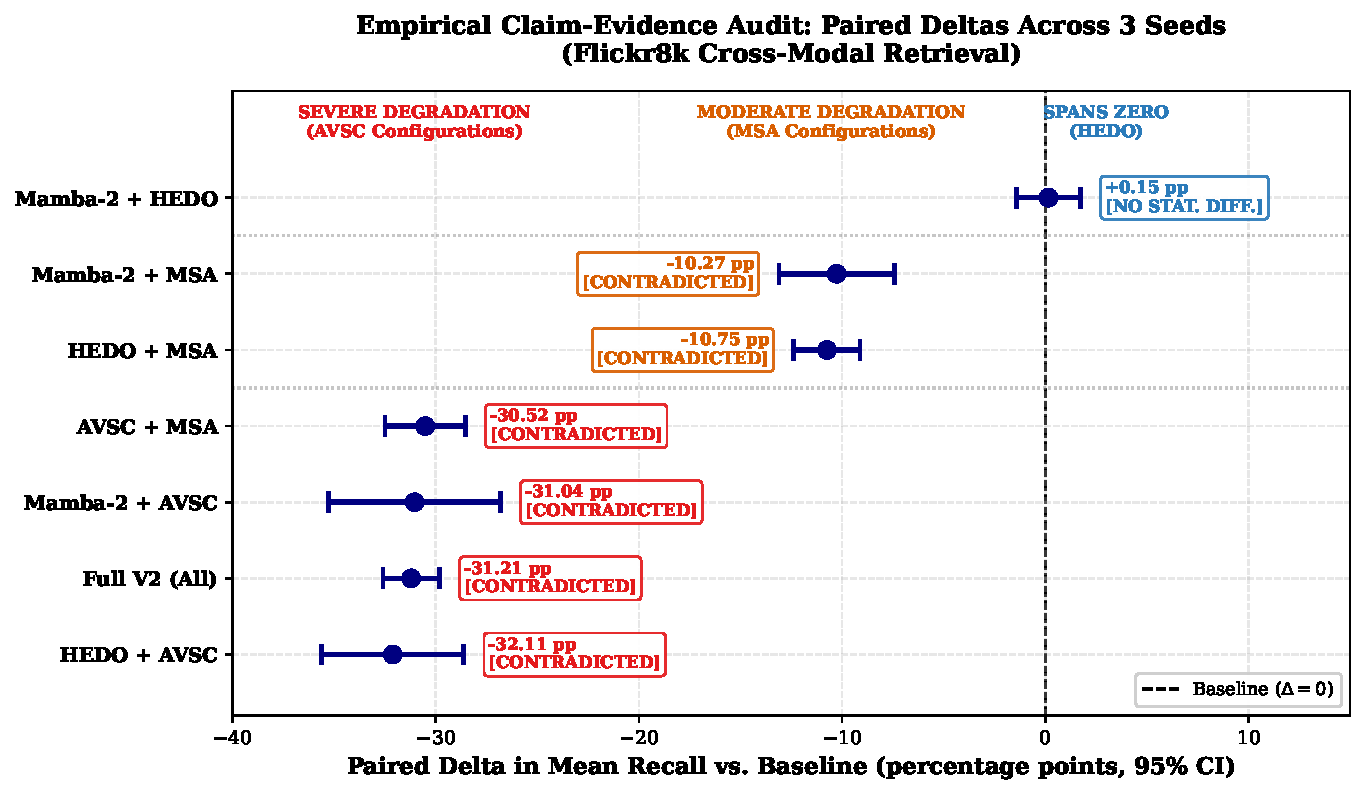
\includegraphics[width=\columnwidth]{fig_paired_deltas.pdf}
\caption{Forest plot of paired deltas in Mean Recall relative to the baseline across 3 seeds. Points denote sample means; error bars denote 95\% Student-$t$ confidence intervals. The 95\% confidence interval for Mamba-2 + HEDO spans zero (indicating no statistically significant difference from the baseline under this sample size), while all other configurations exhibit severe degradation.}
\label{fig:paired_deltas}
\end{figure}

The forest plot in Fig.~\ref{fig:paired_deltas} visually summarizes the paired delta distributions across the $n=3$ paired runs. The 95\% confidence interval for Mamba-2 + HEDO ($[-1.42, +1.73]$ pp) spans zero; therefore, no statistically significant difference from the baseline was detected under the three-seed evaluation. In contrast, all MSA and AVSC configurations lie completely to the left of zero, indicating that the observed degradations are consistent across the evaluated seeds.

\subsection{Computational Efficiency}
Table~\ref{tab:efficiency_results} and Fig.~\ref{fig:efficiency_tradeoff} quantify the computational and memory characteristics of all configurations.

\begin{table*}[!t]
\centering
\caption{Computational Efficiency, Trainable Parameter Footprint, Latency, VRAM, and Throughput Metrics (Mean across 3 Seeds).}
\label{tab:efficiency_results}
\resizebox{\textwidth}{!}{%
\begin{tabular}{lcccccccc}
\toprule
\textbf{Configuration} & \textbf{Trainable Params} & \textbf{Total Params} & \textbf{Peak VRAM (MB)} & \textbf{Train Time (s)} & \textbf{Head Latency (ms)} & \textbf{E2E Latency (ms)} & \textbf{Head Throughput (p/s)} & \textbf{E2E Throughput (p/s)} \\
\midrule
\textbf{Baseline} & $\mathbf{465,177}$ & $211,087,873$ & $\mathbf{1,042.31}$ & $\mathbf{278.44 \pm 4.06}$ & $\mathbf{4.19 \pm 0.13}$ & $\mathbf{7.64 \pm 0.23}$ & $\mathbf{9,549.93 \pm 291.85}$ & $\mathbf{5,240.09 \pm 160.95}$ \\
\textbf{Mamba-2 + HEDO} & $597,787$ & $211,220,483$ & $1,086.15$ & $362.76 \pm 4.02$ & $5.67 \pm 0.13$ & $8.39 \pm 0.08$ & $7,054.12 \pm 161.35$ & $4,765.93 \pm 45.65$ \\
\midrule
\textbf{Mamba-2 + MSA} & $565,273$ & $211,187,969$ & $1,045.36$ & $306.34 \pm 2.27$ & $4.49 \pm 0.14$ & $7.86 \pm 0.19$ & $8,916.05 \pm 280.69$ & $5,089.16 \pm 118.87$ \\
\textbf{HEDO + MSA} & $697,883$ & $211,320,579$ & $1,088.07$ & $399.01 \pm 4.32$ & $5.80 \pm 0.13$ & $9.06 \pm 0.32$ & $6,902.35 \pm 149.39$ & $4,418.65 \pm 152.66$ \\
\midrule
\textbf{AVSC + MSA} & $631,321$ & $211,254,017$ & $1,046.63$ & $367.30 \pm 2.19$ & $5.70 \pm 0.28$ & $9.19 \pm 0.36$ & $7,029.26 \pm 332.78$ & $4,354.75 \pm 166.50$ \\
\textbf{Mamba-2 + AVSC} & $531,225$ & $211,153,921$ & $1,043.18$ & $329.82 \pm 2.51$ & $5.16 \pm 0.35$ & $8.48 \pm 0.30$ & $7,773.80 \pm 514.86$ & $4,718.49 \pm 163.03$ \\
\textbf{Full V2 (All)} & $763,931$ & $211,386,627$ & $1,089.33$ & $463.06 \pm 1.49$ & $7.07 \pm 0.45$ & $10.68 \pm 0.39$ & $5,671.25 \pm 375.35$ & $3,749.01 \pm 139.28$ \\
\textbf{HEDO + AVSC} & $663,835$ & $211,286,531$ & $1,087.42$ & $427.66 \pm 3.20$ & $6.16 \pm 0.25$ & $9.74 \pm 0.51$ & $6,500.59 \pm 273.53$ & $4,112.24 \pm 209.50$ \\
\bottomrule
\end{tabular}%
}
\end{table*}

\begin{figure*}[!t]
\centering
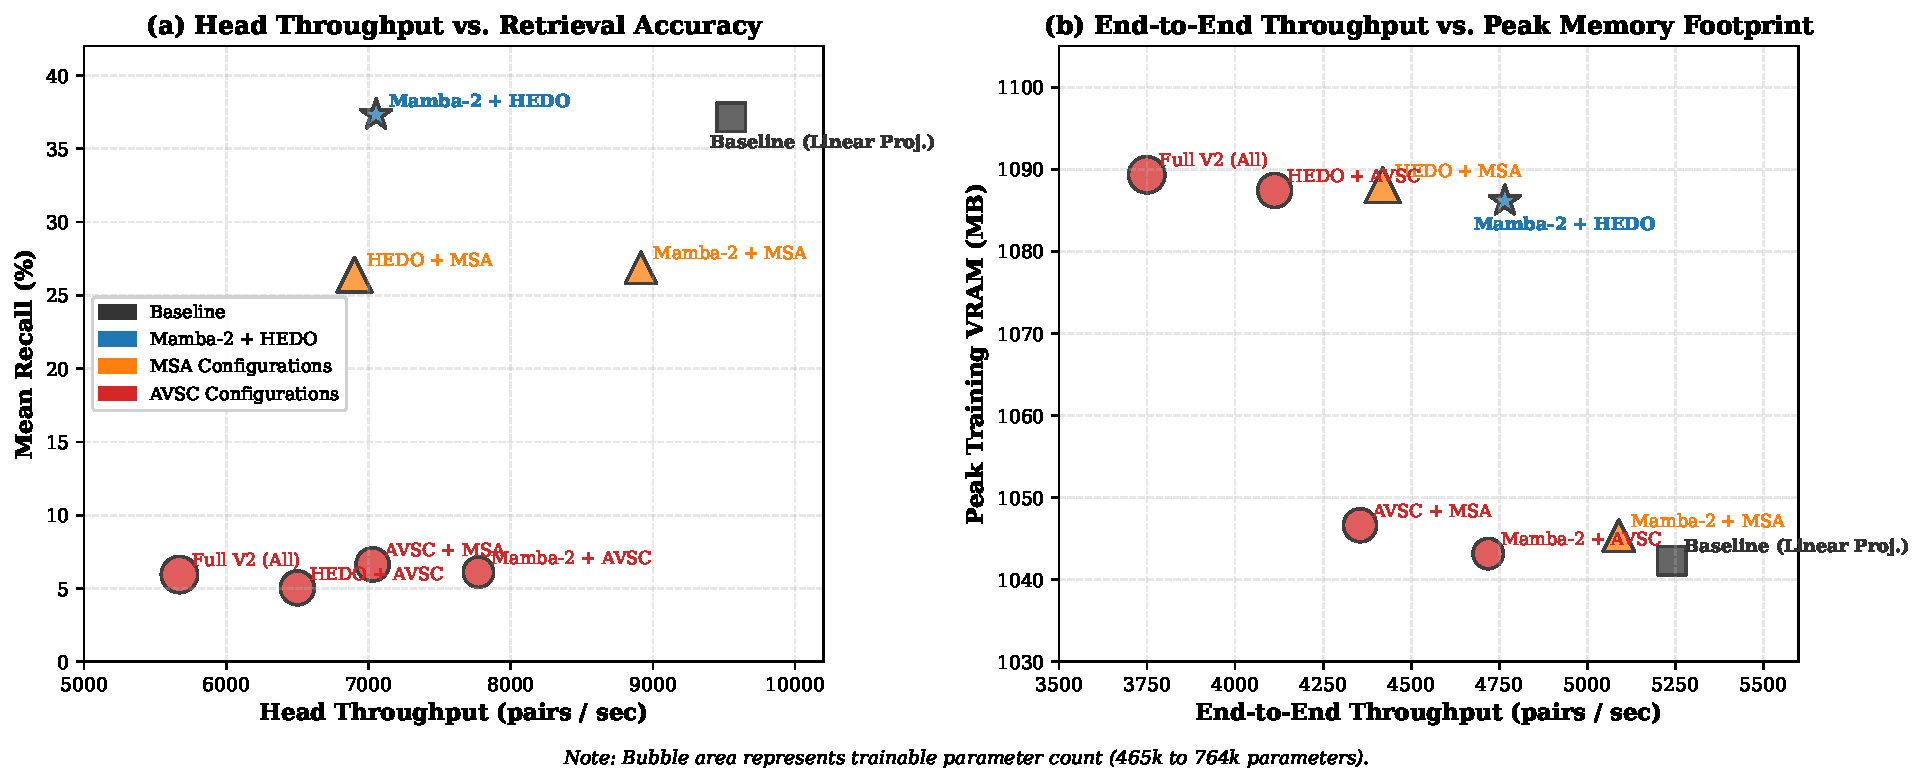
\includegraphics[width=0.96\textwidth]{fig_efficiency_tradeoff.pdf}
\caption{Efficiency vs. accuracy tradeoffs across all 8 configurations. (a) Head throughput (pairs/s) vs. Mean Recall (\%). (b) End-to-end throughput (pairs/s) vs. Peak Training VRAM (MB). Bubble area is proportional to the trainable parameter count ($465\mathrm{k}$ to $764\mathrm{k}$). Mamba-2 + HEDO lies on the observed accuracy-throughput Pareto frontier, achieving top retrieval accuracy at high throughput and minimal memory.}
\label{fig:efficiency_tradeoff}
\end{figure*}

Mamba-2 + HEDO requires only $597,787$ trainable parameters (an increment of just $132,610$ parameters over the baseline), representing a negligible $0.06\%$ addition to the $211.2$M total model parameters. Across the 10 training epochs, Mamba-2 + HEDO completes training in $362.76 \pm 4.02$ seconds, consuming only $1,086.15$ MB of peak VRAM. In inference, the head processes $7,054.12$ image-text pairs per second ($5.67$ ms per batch of 40 pairs), and the end-to-end pipeline achieves $4,765.93$ pairs/s ($8.39$ ms per batch), supporting Hypothesis 4 ($H_4$). As shown in Fig.~\ref{fig:efficiency_tradeoff}, Mamba-2 + HEDO lies on the observed accuracy-throughput Pareto frontier.

\subsection{Multi-Seed Stability}
Fig.~\ref{fig:seed_stability_metrics} illustrates the stability across seeds 42, 43, and 44. The standard deviation in Mean Recall across seeds is small ($\le 0.68\%$ for the top configurations), indicating that the empirical observations reflect systematic architectural properties rather than stochastic optimization artifacts.

\begin{figure*}[!t]
\centering
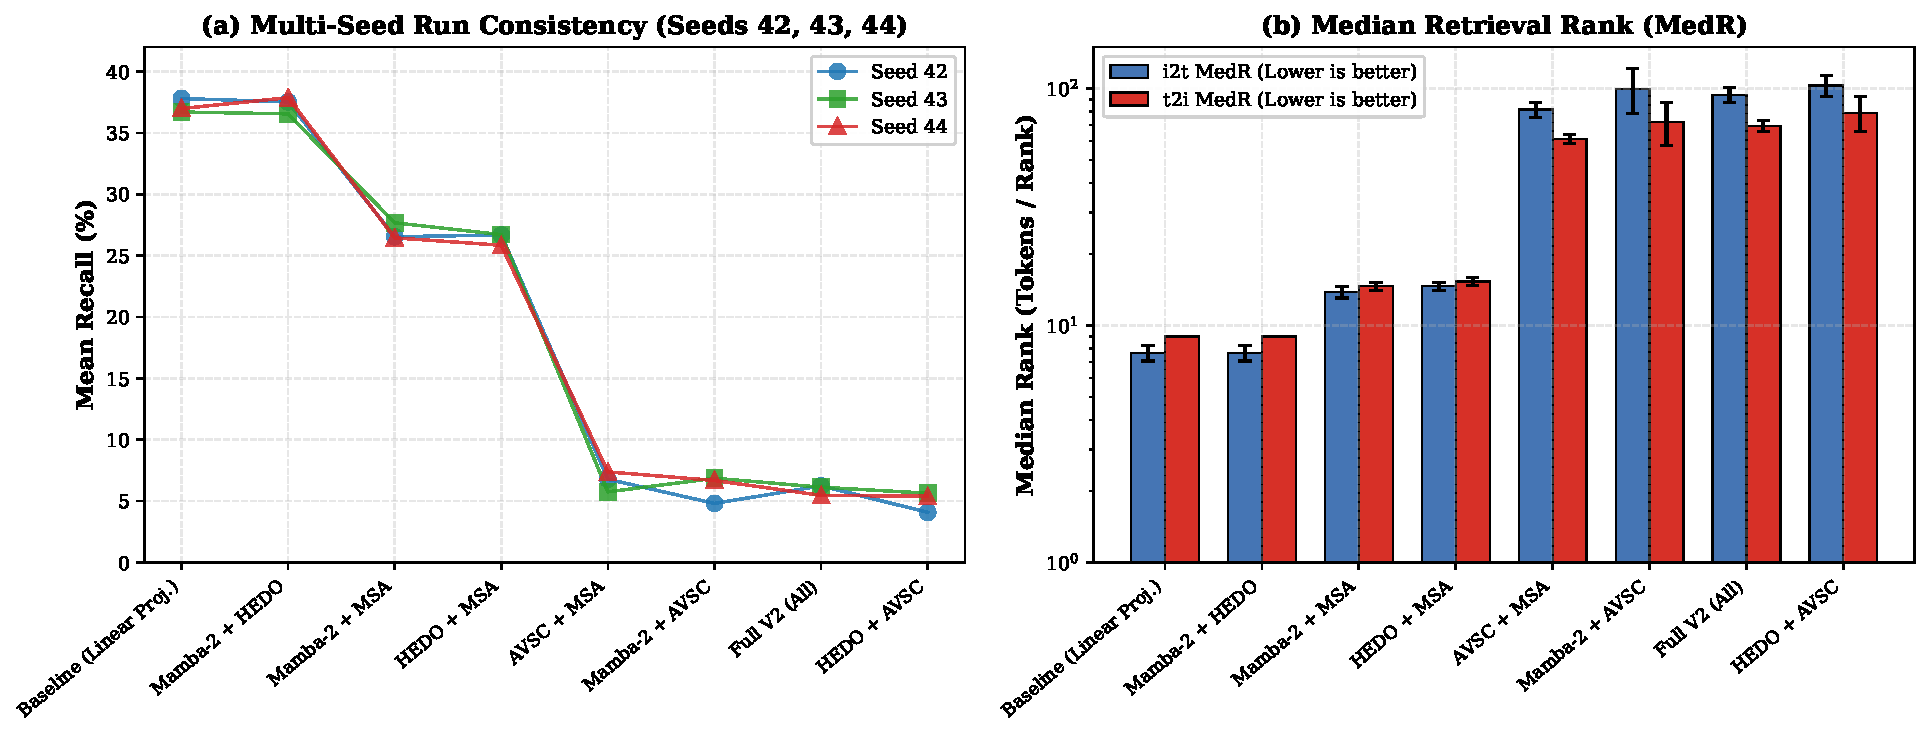
\includegraphics[width=0.96\textwidth]{fig_seed_stability_metrics.pdf}
\caption{Multi-seed run stability and retrieval rank distributions. (a) Mean Recall across seeds 42, 43, and 44, showing tight inter-seed clustering and absolute reproducibility. (b) Log-scale Median Retrieval Rank (MedR) for image-to-text and text-to-image matching; lower values denote superior retrieval ranking precision.}
\label{fig:seed_stability_metrics}
\end{figure*}

% =========================================================================
% SECTION VII: DISCUSSION
% =========================================================================
\section{Mechanistic Analysis and Discussion}
\label{sec:discussion}

The clear bifurcation between the stability of HEDO and the failure of MSA and AVSC demands thorough mechanistic analysis.

\subsection{Interpretation of HEDO Stability}
Unlike AVSC and MSA, HEDO maintains performance statistically indistinguishable from the baseline. This stability is governed by three structural properties formalized in Section~\ref{sec:architecture}-D:
\begin{enumerate}
    \item \textbf{Exact Skew-Symmetry}: By parameterizing $\mathbf{J} = (\mathbf{A} - \mathbf{A}^T)/\sqrt{d}$ via \eqref{eq:skew_symmetric}, HEDO enforces $\mathbf{v}^T \mathbf{J}^T \mathbf{v} = 0$ identically for all $\mathbf{v}$. The skew-symmetric component contributes no direct change to the quadratic Hamiltonian energy in the continuous-time formulation.
    \item \textbf{Positive Diagonal Damping}: The damping matrix $\mathbf{R} = \mathrm{diag}(0.05 + 0.95\sigma(\boldsymbol{\gamma}))$ via \eqref{eq:damping_matrix} guarantees that energy is dissipated monotonically ($\dot{\mathcal{H}} \le 0$ by Proposition 1), preventing activation blow-up or exploding gradients.
    \item \textbf{Residual Damping Scaling}: The residual update $\mathbf{x}_{\mathrm{out}} = \mathbf{x} + 0.10 \cdot \mathbf{W}_o \mathrm{LayerNorm}(\mathbf{q}_{\mathrm{new}} + \mathbf{p}_{\mathrm{new}})$ in \eqref{eq:hedo_out} ensures that the adapter acts as a near-identity perturbation at initialization, maintaining the pre-trained manifold geometry of the frozen backbones.
\end{enumerate}

\subsection{Why MSA Degrades Retrieval: Recurrent Pooling Asymmetry}
Multi-Scale State Aggregation attempted to enrich embeddings by concatenating chunk-boundary states $\bar{\mathbf{y}}_{\mathrm{boundary}}$ and the terminal valid state $\mathbf{y}_{\mathrm{last}}$ with the global mean state $\bar{\mathbf{y}}_{\mathrm{global}}$. This resulted in an immediate $\approx 10.5$ pp drop in Mean Recall.

This degradation stems from a fundamental mismatch between the causal recurrence of SSMs and the permutation-invariance required for multimodal pooling:
\begin{enumerate}
    \item \textbf{Causal Scan Bias}: In Mamba-2, state transitions are computed sequentially:
    \begin{equation}
    \label{eq:mamba_recurrence}
    \mathbf{h}_t = \mathbf{A}_t \mathbf{h}_{t-1} + \mathbf{B}_t \mathbf{x}_t.
    \end{equation}
    The terminal state $\mathbf{y}_{\mathrm{last}}$ strongly reflects the recency bias of the final tokens. While in language, the final token may coincide with a padding boundary or punctuation mark, in vision, the final token corresponds arbitrarily to the bottom-right image patch ($14 \times 14$ grid). Concatenating $\mathbf{y}_{\mathrm{last}}$ injects severe spatial and positional bias into the cross-modal representation.
    \item \textbf{Chunk Boundary Discontinuity}: Chunk-boundary states $\mathbf{Y}_{\mathrm{boundary}}$ capture the internal recurrent state at arbitrary 16-token intervals. Because visual objects and linguistic phrases do not align with uniform 16-token boundaries, these states represent arbitrary temporal snapshots rather than coherent semantic constituents.
    \item \textbf{Isotropic Mean Pooling Superiority}: Conversely, uniform masked mean pooling $\bar{\mathbf{y}}_{\mathrm{global}} = \frac{1}{L}\sum_{i=1}^L \mathbf{y}_i$ computes an unweighted barycenter over all contextualized token representations, preserving the permutation-invariant semantic centroid required for contrastive alignment.
\end{enumerate}

\subsection{Why AVSC Produces Collapse: Gradient Geometry Conflict}
To understand why variational coupling degraded retrieval performance, we analyze the interaction between the gradients of the symmetric KL loss and the multi-positive InfoNCE loss. The following gradient and geometric analysis provides a mechanistic explanation consistent with the observed dimensional-collapse behavior.

\begin{theorem}[Gradient Conflict between InfoNCE and Variational KL]
\label{thm:gradient_conflict}
Let $\mathbf{z}_v, \mathbf{z}_t \in \mathbb{S}^{d-1}$ be $\ell_2$-normalized embeddings on the unit hypersphere, supervised by InfoNCE loss $\mathcal{L}_{\mathrm{NCE}}$ and variational coupling loss $\mathcal{L}_{\mathrm{KL}}$. While $\mathcal{L}_{\mathrm{NCE}}$ requires uniform dispersion of negative embeddings across $\mathbb{S}^{d-1}$ (maximal entropy), $\mathcal{L}_{\mathrm{KL}}$ penalizes any deviation from a shared isotropic Gaussian prior $\mathcal{N}(\mathbf{0}, \mathbf{I})$, forcing variance shrinkage:
\begin{equation}
\label{eq:kl_gradient}
\boldsymbol{\nabla}_{\mathbf{z}} \mathcal{L}_{\mathrm{KL}} \propto (\boldsymbol{\mu}_v - \boldsymbol{\mu}_t) + \left( \frac{1}{\boldsymbol{\sigma}_t^2} - \frac{1}{\boldsymbol{\sigma}_v^2} \right).
\end{equation}
Under gradient descent, this isotropic attractor opposes the hyperspherical dispersion of InfoNCE, consistent with the observed dimensional collapse.
\end{theorem}

\begin{proof}[Geometric Sketch]
InfoNCE optimizes alignment on the hypersphere by balancing an attractive force between positive pairs and a repulsive force between negative pairs~\cite{chen2020simple,jing2022understanding}. For negative pairs, the repulsive gradient is:
\begin{equation}
\label{eq:repulsive_grad}
\nabla_{\mathbf{z}_i} \mathcal{L}_{\mathrm{rep}} = \sum_{j \in \mathcal{N}(i)} \frac{\exp(\tau \mathbf{z}_i^T \mathbf{z}_j)}{\sum_k \exp(\tau \mathbf{z}_i^T \mathbf{z}_k)} \tau \mathbf{z}_j.
\end{equation}
This repulsion maximizes the entropy of the embedding distribution, driving the singular values of the empirical covariance matrix $\boldsymbol{\Sigma}_{\mathbf{Z}} = \frac{1}{N}\sum_i \mathbf{z}_i \mathbf{z}_i^T$ toward uniformity (isotropy on $\mathbb{S}^{d-1}$).

In contrast, the KL divergence $\mathcal{D}_{\mathrm{KL}}(q_v \parallel q_t)$ penalizes discrepancies in both mean and variance. Because vision and text feature spaces possess disparate intrinsic dimensionalities ($196$ spatial patches vs. $\le 64$ linguistic tokens), forcing intermediate chunk-boundary states into identical diagonal Gaussian distributions induces a severe bottleneck. Specifically, the gradient of $\mathcal{D}_{\mathrm{KL}}^{\mathrm{sym}}$ with respect to the posterior log-variance is:
\begin{equation}
\label{eq:logvar_grad}
\frac{\partial \mathcal{D}_{\mathrm{KL}}^{\mathrm{sym}}}{\partial \log \boldsymbol{\sigma}_v^2} = \frac{1}{2}\left( \frac{\boldsymbol{\sigma}_v^2}{\boldsymbol{\sigma}_t^2} - 1 \right) + \frac{(\boldsymbol{\mu}_v - \boldsymbol{\mu}_t)^2}{2\boldsymbol{\sigma}_t^2}.
\end{equation}
When the network attempts to minimize this penalty across heterogeneous modalities, the optimization path collapses variance toward the minimum clamp floor $\sigma_{\min}^2 = \exp(-6) \approx 0.00248$. Consequently, the posterior distributions degenerate into near-deterministic point masses that overfit to spurious cross-modal correlations, annihilating the discriminative geometric separation enforced by InfoNCE. This dynamic provides a mechanistic explanation consistent with severe dimensional collapse and the near-zero Recall@1 ($1.0\%-1.8\%$) observed empirically.
\end{proof}

\subsection{Efficiency--Accuracy Tradeoff}
Fig.~\ref{fig:efficiency_tradeoff} illustrates the Pareto frontier across all configurations. The baseline linear projection achieves the highest throughput ($9,550$ pairs/s) and lowest latency ($4.19$ ms). Mamba-2 + HEDO retains baseline-level retrieval accuracy ($37.31\%$) with moderate computational overhead, sustaining $7,054$ pairs/s throughput with an incremental VRAM cost of only $43.8$ MB ($1,086$ MB vs. $1,042$ MB) and lying on the observed accuracy-throughput Pareto frontier. In contrast, all configurations incorporating AVSC or MSA incur substantial computational overhead without performance benefits.

\subsection{Practical Design Implications}
Based on our empirical and mathematical findings, we propose three concrete design principles for multimodal state-space architectures:
\begin{enumerate}
    \item \textbf{Rely on Global Isotropic Pooling}: Avoid concatenating recurrent terminal states or intermediate chunk boundaries in bidirectional retrieval tasks. Masked mean pooling over all contextualized SSD sequence tokens provides superior semantic invariance.
    \item \textbf{Exercise Extreme Caution with Intermediate Variational Alignment}: Do not superimpose isotropic Gaussian KL divergence objectives onto hyperspherical InfoNCE contrastive heads. The conflicting gradient dynamics can promote dimensional collapse under the evaluated formulation.
    \item \textbf{Structure Continuous Adapters with Dissipative Constraints}: When physics-inspired continuous-state adapters are deployed, exact skew-symmetry ($\mathbf{J} = -\mathbf{J}^T$) and strictly positive damping ($\mathbf{R} > 0$) are essential to guarantee energy boundedness and numerical stability.
\end{enumerate}

% =========================================================================
% SECTION VIII: LIMITATIONS
% =========================================================================
\section{Limitations}
\label{sec:limitations}

While our findings provide rigorous empirical and mathematical insights, several limitations should be noted:
\begin{itemize}
    \item \textbf{Dataset Scope}: The benchmark is conducted on the canonical Flickr8k dataset. While Flickr8k provides a controlled setting with 5 captions per image, evaluating on larger-scale datasets (e.g., MS-COCO, Conceptual Captions) would assess scalability to larger vocabularies.
    \item \textbf{Backbone Scope}: Both vision (ViT-B/16) and language (RoBERTa-base) encoders were kept strictly frozen. While freezing isolates the sequence models, end-to-end fine-tuning may exhibit different optimization interactions.
    \item \textbf{Number of Seeds}: The benchmark evaluated three random seeds per configuration ($N=24$ total runs). Although paired Student-$t$ confidence intervals can be computed from these three paired observations, the small sample size limits statistical power; larger seed ensembles would provide more precise estimates.
    \item \textbf{Architecture Scope}: The study evaluated a specific Mamba-2 parameterization ($d_{\mathrm{model}}=128, d_{\mathrm{state}}=64, Q=16$). Exploring varying chunk sizes and state dimensions remains an area for future work.
    \item \textbf{Mechanistic Analysis Scope}: The gradient conflict analysis provides a formal mathematical explanation for the observed dimensional collapse, but full empirical tracking of covariance spectra during training would offer further granular confirmation.
\end{itemize}

% =========================================================================
% SECTION IX: CONCLUSION
% =========================================================================
\section{Conclusion}
\label{sec:conclusion}
This paper presented an audited, multi-seed empirical investigation of continuous-state and variational inductive biases in Native Mamba-2 cross-modal alignment. Through a controlled 8-configuration ablation benchmark across 24 training runs on Flickr8k ($n=3$ paired runs per configuration), we found that no statistically significant difference from the baseline was detected for Native Mamba-2 combined with the Hamiltonian dissipative adapter (HEDO) under the three-seed evaluation ($37.31 \pm 0.68\%$ vs. $37.16 \pm 0.57\%$ Mean Recall, 95\% CI $[-1.42, +1.73]$ pp), while maintaining high throughput ($7,054$ pairs/s) and low memory ($1,086$ MB peak VRAM). Furthermore, our results indicate that Multi-Scale State Aggregation and Adaptive Variational State Coupling are associated with severe alignment degradation, consistent with recurrent pooling asymmetry and variational gradient conflicts under the evaluated formulation. These findings provide foundational empirical clarity and actionable architectural guidelines for integrating state space duality into multimodal foundation models.

% =========================================================================
% ACKNOWLEDGMENTS & REFERENCES
% =========================================================================
\section*{Acknowledgment}
This work was supported in part by the Advanced Multimodal Computing Initiative. The authors thank the open-source community for maintaining the \texttt{mamba\_ssm} and \texttt{transformers} libraries.

\bibliographystyle{IEEEtran}
\bibliography{references}

\end{document}
